\chapter{自动化线虫视频分析与特征提取}
\section{引言}
	在基于线虫的毒理实验中,通常需要观察在给药的过程中线虫生理特征的变化,如在基于线虫的神经毒性实验中
	需要对线虫的存活率、身体弯曲频率、头部摆动频率等特征进行统计。在基于线虫的发育毒性实验中,需要对
	线虫的身体长度、形状、产卵器形态发育等特征进行统计。在基于线虫的生殖毒性实验中需要对线虫的胚胎发育、
	性腺形态发育、后代数目进行统计观察。通过人工观察的方式不仅会引入误差,而且效率低下。由于实验数据分析
	上存在瓶颈的情况,严重限制了实验的规模。因此,线虫的自动化视频分析和特征提取对于大规模的毒理实验和药
	物筛选是至关重要的。
	
	针对线虫自动化视频分析和特征提取任务的特点,
	本文采用了“前景轮廓分割——轮廓解析——轮廓跟踪——特征提取”的技术路线。
	其中前景轮廓分割和轮廓解析是整个技术路线中关键的一步,其结果直接影响到能否对线虫进行有效的跟踪以及特征提取
	等后续步骤。线虫轮廓分割的不完整会导致跟踪的丢失率显著上升。为了提高线虫轮廓分割的精度,本章将深度卷积网络
	应用在线虫前景轮廓分割和轮廓解析任务中,并与传统的分割算法做了详细的比较分析。发现基于深度卷积网络的分割
	算法能够显著地改善线虫前景轮廓分割的效果。为了实现对线虫轮廓的跟踪,本章提出了一种基于最近邻搜索的跟踪方法
	,在线虫轮廓分割较为完整的情况下,能够实现对线虫的鲁棒跟踪。最后,介绍了线虫体长和摆动频率等特征的计算方法。

\section{线虫图像处理总体方案介绍}
	图\ref{fig:flow}显示了线虫视频特征提取的技术路线流程,共分成四个阶段。
	第一个阶段为线虫前景轮廓的分割,从采集的视频中读取一帧图像,并将
	线虫轮廓覆盖的区域定义为前景,剩下的区域视为背景。利用图像分割算法进行前景背景分割后得到一幅二值化的图像,
	其中1表示前景0表示背景。如果是单线虫的跟踪,则第一个阶段的输出则为线虫的轮廓。
	但考虑到多线虫跟踪过程中多个线虫的轮廓会出现
	相交甚至纠缠在一起,导致因无法区分单个线虫轮廓从而跟踪丢失。第二个阶段的任务是对多个纠缠在一起的线虫轮廓进行解析,
	从而得到单个线虫的轮廓。第三个阶段是线虫轮廓的跟踪,利用线虫轮廓的重心、面积等信息找出相邻两帧图像之间线虫轮廓的对应
	关系。第四个阶段为线虫特征计算,利用上一阶段跟踪的线虫轮廓计算线虫体长、运动速度和摆动频率等生理特征。
	本章的剩余部分将依次对各个部分进行介绍。
	\begin{figure}[!htp]
    \centering
    \begin{tikzpicture}[node distance=2.5cm,auto]
	\tikzstyle{rect1} = [rectangle,rounded corners,thick,minimum width = 3cm,
	text width=3cm,inner sep=2pt,minimum height =2cm, text centered, draw = black]
    \tikzstyle{rect2} = [rectangle,rounded corners,thick,minimum width = 3cm,fill=orange!30,
	text width=3cm,inner sep=2pt,minimum height =2cm, text centered, draw = black]
	\tikzstyle{label} = [rectangle,rounded corners,minimum width = 7cm,text width=7cm,inner sep=2pt,minimum height =1.5cm, text centered, draw = black]
	\tikzstyle{arrow1} = [->, >=latex', shorten >=1pt, thick]
	\tikzstyle{arrow2} = [->, >=latex', shorten >=1pt]
	\node (node1) [rect1] {线虫前景轮廓分割};
    \node (node2) [rect1, right of=node1,node distance=4cm] {线虫轮廓解析};
    \node (node3) [rect1, right of=node2,node distance=4cm] {线虫轮廓跟踪};
    \node (node4) [rect1, right of=node3,node distance=4cm] {特征计算:线虫体长、面积、摆动频率等};
	%\node (node5) [cylinder,right of=node4,shape border rotate=90,draw,minimum height=3cm,minimum width=2cm]{};

	%连接具体形状
    \draw [arrow1](node1) -- (node2);
    \draw [arrow1](node2) -- (node3);
    \draw [arrow1](node3) -- (node4);
	%\draw {arrow1}(node4) --(node5);
    % \draw [arrow2](node1) -- (label1);
	% \draw [arrow2](node2) -- (label2);
	% \draw [arrow2](node3) -- (label3);
	% \draw [arrow2](node4) -- (label4);
	\end{tikzpicture}
    	  \bicaption
		{线虫图像处理总体流程图}
		{The flow chart of C.elegans image processing}
	  \label{fig:flow}
	\end{figure}

\section{基于深度卷积网络的线虫前景轮廓分割}
秀丽隐杆线虫由于通体透明,且PDMS制作的微流控芯片也是透明的,
所以线虫轮廓的分割是个难点。使用传统的图像分割方法在线虫前
景轮廓分割任务中均表现较差。如通过简单的阈值分割的方法\cite{otsu1979threshold},
并不能够很好地分割线虫的轮廓,因为前景像素的灰度值范围在背景像素的灰度范围内;
通过背景减除的前景背景分割方法\cite{zivkovic2006efficient}也会因为图像噪声的影响,
导致分割的线虫轮廓出现断裂、
不完整等情况。这些情况会导致后续线虫跟踪的丢失率显著上升。另一方面,背景的估计需50$\sim$100帧背景不变的图像。
当需要对线虫进行实时跟踪时,基于背景估计的线虫前景分割算法需要一个启动时间用于背景的估计。
另外,当相机或载物台移动时(如:需要观察不同腔室中的虫子),由于背景的改变,这种算法还是会失效。

卷积网络作为一种强大的特征提取器在许多计算机视觉任务中取得了很大的成功。
本小节,我们针对线虫前景轮廓分割的任务特点,设计了一个基于条件随机场模
型的全卷积网络。并标注了一个线虫前景轮廓分割数据集,
用于对网络的模型参数进行训练。实验结果显示,基于条件随机场模型的全卷积分割
网络的分割性能较好,且具有如下优势:
	
\begin{enumerate}
  \item 满足实时性。与基于背景减除的方法相比,基于卷积网络的分割不需要对图像背景建模,
  只依赖当前帧的图像,从而能够保证实时性的要求。
  \item 能够降低硬件成本。传统的线虫图像分割方法,为了获得一个背景和线虫轮廓对比度比较高的图像,
  通常使用特制的硬件对相机和照明都有很高的要求。卷积网络作为一种强大特征提取器降低了对图像质量的要求。
  \item 鲁棒性更好。传统的图像分割算法,通常需要人工地选取一些超参数(如:分割的阈值,形态学操作中核的大小等等),
  但由于视频采集过程中照明的变化以及图像噪声的影响很难选取一个最佳的全局参数。
基于卷积网络的分割是一种端到端的方法,输出直接是分割的结果。因此,这种方法几乎不依赖超参数的选取,具有很好的鲁棒性。
\end{enumerate}
\subsection{数据集的制作}
\subsubsection{数据集的采集}
	图\ref{fig:chap5:camera}是线虫图像采集的系统装置图,主要由显微镜、DigiRetina 16 COMS相机、照明系统和微流控芯片四个部分组成,DigiRetina 16
	相机通过数据线连接电脑进行图像数据传输。线虫通过压力进样地方式注入到微流控芯片的腔室内。移动显微镜的载物台使线虫腔室
	位于视野的正中央。调节显微镜的放大倍数使线虫腔室充满整个视野。调整显微镜焦距使视野中呈现清晰的图像。调整相机的
	曝光时间以获得一个对比度比较高的线虫图像。完成以上步骤后便可以进行线虫视频的采集。
	\begin{figure}[thb]
	  \centering
	  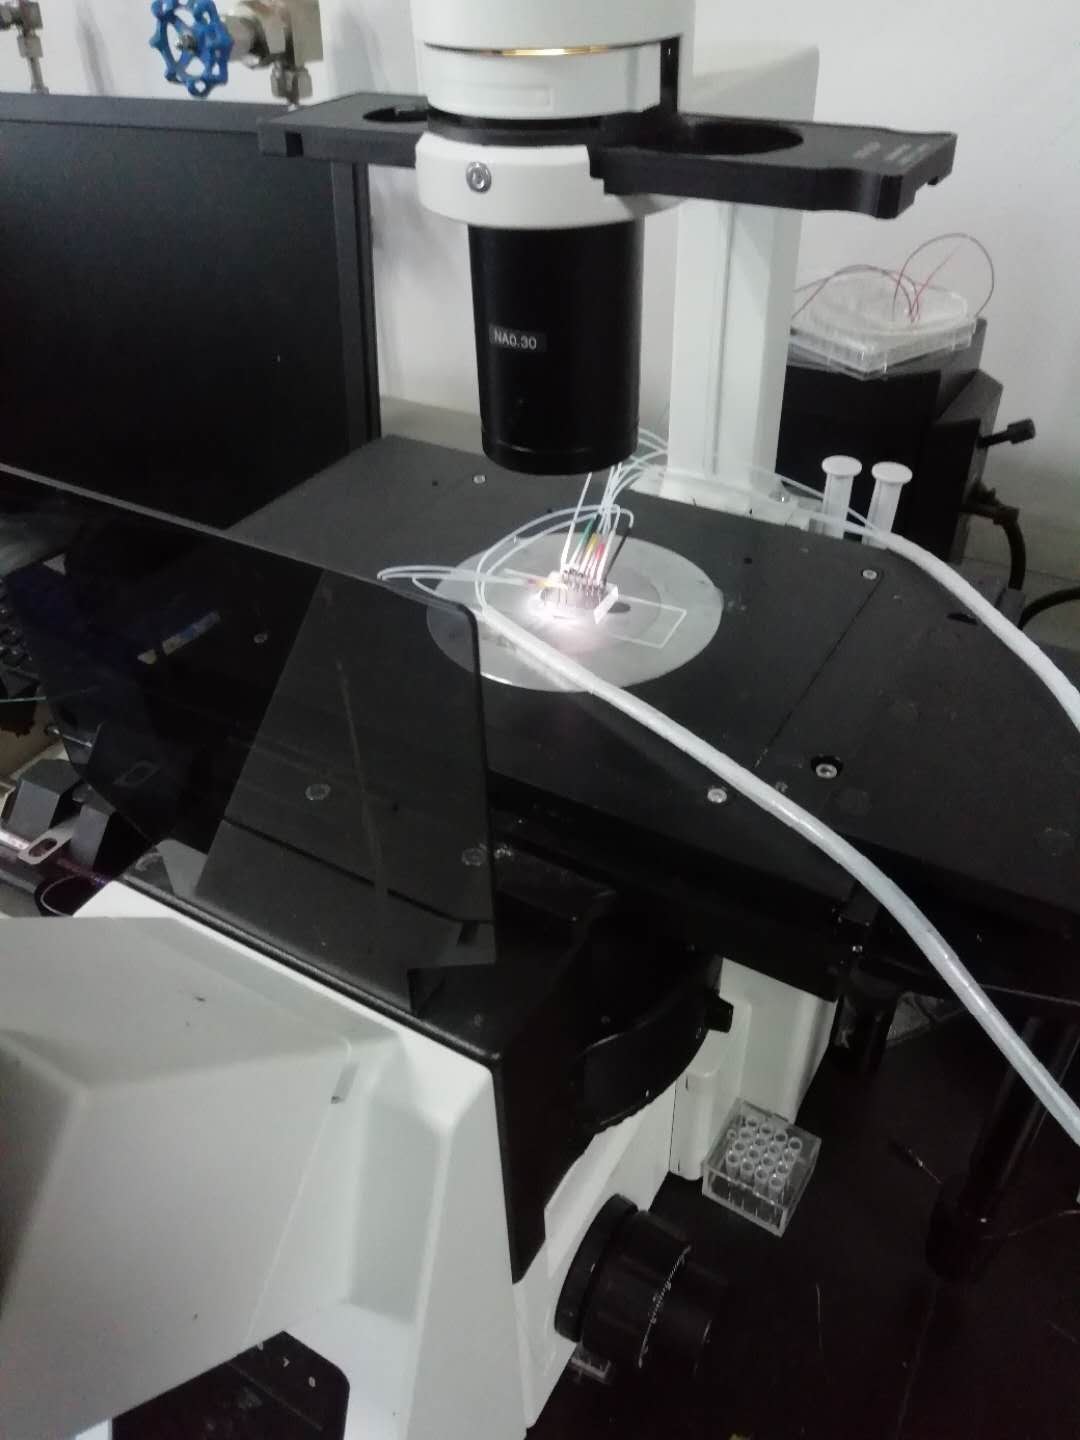
\includegraphics[width=8cm]{figure/chap5/camera.jpg}
	  \bicaption
		{图像采集系统装置图}
		{System diagram of image acquisition}
	  \label{fig:chap5:camera}
	\end{figure}
\subsubsection{数据集的标注}
	高质量的数据集对网络的训练来说至关重要,且数据集的质量决定了神经网络模型性能的上限,通过优化网络架构的方法
	也只能逼近这个上限。但数据集的标注通常是一个非常耗时的过程,特别是图像分割任务要对不同的区域标记。目前很多的
	图像分割标注工具(如:Labelme\footnote{\url{https://github.com/wkentaro/labelme}}和Ratesnake\footnote{\url{https://is-innovation.eu/ratsnake/}}等)都是采用多边形近似的标注方法,
	即在轮廓的四周边缘采集足够多的点,这些点构成的多边形为标注对象的轮廓。由于线虫形态变化复杂,相对于其他目标
	的标注往往需要采集更加密集的点才能满足线虫轮廓标注的精度。为了提高线虫图像标注的效率,本文采用了一种半自动的线虫轮廓
	标注方法。将Grabcut算法用于线虫轮廓的标注,只需要用矩形框将线虫轮廓框出作为Grabcut算法输入,算法可以自动的分割
	出线虫的轮廓,最后再将多个线虫轮廓合成为一个标签图像。通过这种方法,本文制作了一个包含236个样本的数据集,图\ref{fig:dataset}是数据集部分示例。
	整个数据集按照$8:2$的比例将其分为训练集与测试集两部分分别用于网络模型的训练与测试。
	\begin{figure}[h]
	  \centering
	  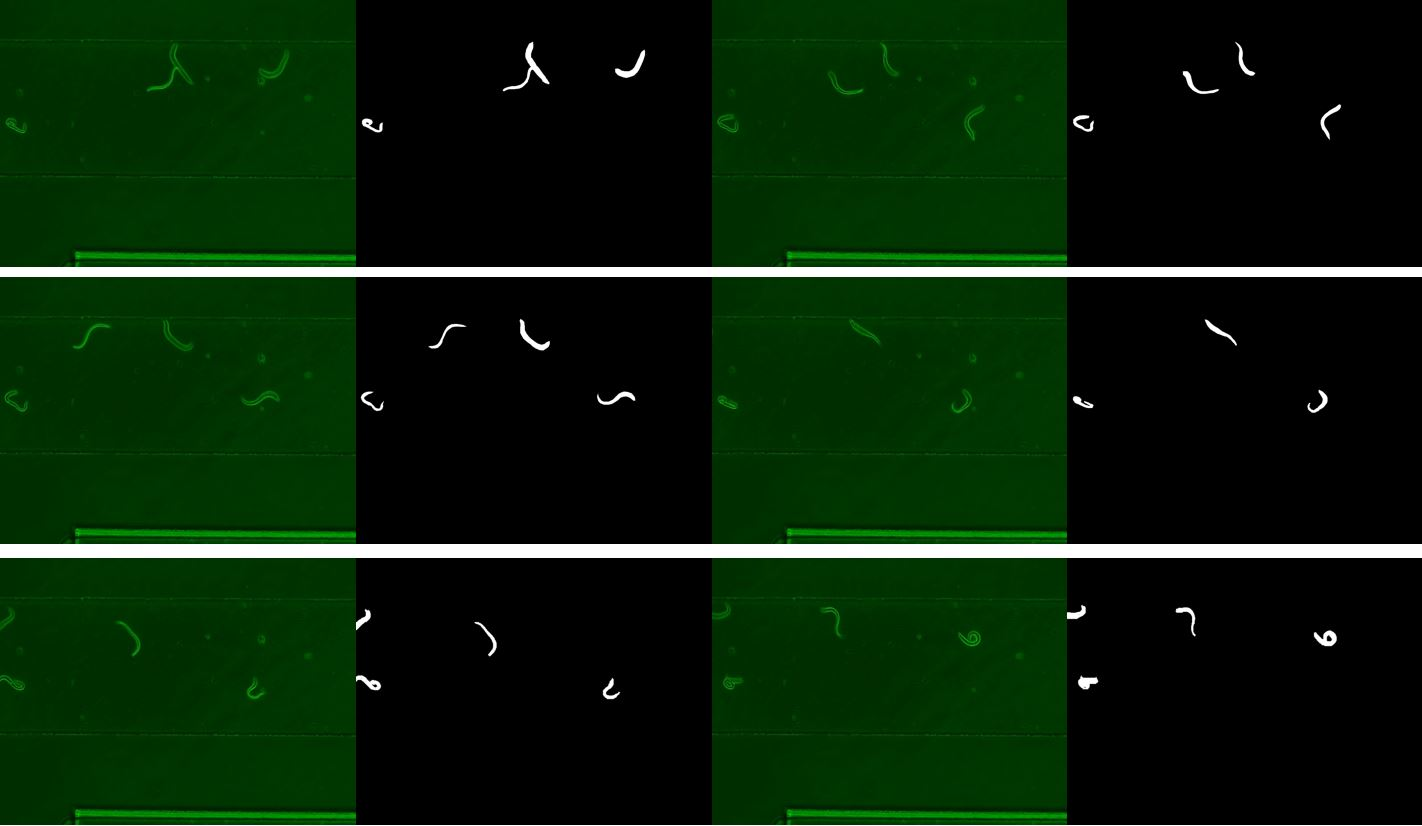
\includegraphics[width=14cm]{figure/chap3/dataset.jpg}
	  % \hspace{1cm}
	  % 
\includegraphics[width=4cm]{example/sjtulogo.jpg}
	  \bicaption
		{线虫前景轮廓分割数据集示例}
		{The image examples from C.elegans foreground segmentation dataset}
	  \label{fig:dataset}
	\end{figure}
\subsection{条件随机场模型在分割任务中的应用}
	条件随机场(Condition random field, CRF)是概率无向图模型中的一种\cite{李航2012统计学习方法},
	目前被很多研究者用于解决图像分割问题并取得了很大的成功\cite{zheng2015conditional,wang2017adaptive,chen2018deeplab}。
	其能够对空间中相邻像素之间的关系进行建模,从而可以得到具有空间一致性和更加精细化的分割结果。
	如果分割算法没有考虑到相邻像素之间的依赖关系,相当于认为空间中每个像素都是独立的,
	这样会导致分割结果中被分割对象的不连续以及可能丢失掉很多细节结构。本文将条件随机场模型应用于
	线虫前景轮廓的分割任务中,并通过卷积模块加以实现,这样可以保证整个模型的可微性。
		
	线虫图像的前景背景分割问题本质上是一个二分类问题,假设有一个标签$Y=\{Y_1,Y_2,\cdots,Y_N\}$
	,$N$表示总的像素,$Y_i\in\{0,1\}$则标签$Y$总共有$2^N$种取值。在$Y$的所有取值中,概率最大对应的取值
	即为最优分割的结果。图像分割问题被转化为基于条件随机场的最大条件概率问题。根据吉布斯分布与条件随机场
	的等效性\cite{Lafferty2001Conditional},定义如下基于标签$Y$的能量函数:
	\begin{equation}
		E(Y|I) = \sum_{l}Y_lU(l)+\sum_{l,k}Y_lW_{l,k}Y_k
	\end{equation}
	其中一元项$U(l)=g(h,l)$表示第$l$个像素标签$Y_l$取值为1的损失,$h$表示图像特征,$W_{l,k}$表示标签$Y_l$和
	标签$Y_k$同时出现的权重。给定一幅线虫图像$I$,对应的标签为Y的条件概率为:
	\begin{equation}
		P(Y|I)=\frac{1}{Z}\exp(-E(Y|I))
	\end{equation}
	其中$Z$为归一化项。通过平均场近似\cite{zheng2015conditional}的方法,标签$Y_l=1$可以通过以下迭代的方法求出:
	\begin{equation}
		\Phi(Y_l=1)_t=\sigma\Big(U(l)+\sum_{k}W_{l,k}\Phi(Y_k=1)_{t-1}\Big)
	\end{equation}
	其中$\Phi(Y_l=1)$表示$Y_l$取值为1的概率,$\sigma(a)=1/(1+\exp(-a))$表示 sigmoid 函数。$U(l)$通过基于图像特征$h$的卷积获得。
	$\sum_{k}W_{l,k}\Phi(Y_k=1)_{t-1}$是通过$t-1$阶段的概率图$\Phi_{t-1}$与卷积核$W$的卷积操作实现的。在$t$时刻的概率图$\Phi_t$可以由如下公式计算:
	\begin{equation}
		\Phi_t=\mathscr{M}(U,W^k)=\begin{cases}
						\sigma(W^k*U), \quad \quad \quad t=0\\
						\sigma(W^k*\Phi_{t-1}+U), \quad t=1,2,3
						\end{cases}
	\end{equation}
	其中$\mathscr{M}$表示基于共享权重的递归卷积,$W^k$表示共享卷积核,其可以对相邻像素之间的空间
	关系进行建模。本文中,我们使用了3次递归卷积实现条件随机场的近似。
	
	
\subsection{网络结构的设计}
\label{subsec:arch-design}
	本文提出了一种用于线虫前景轮廓分割的基于条件随机场的卷积网络模型,图\ref{fig:chap5:arch}为对应的网络架构。
	在卷积分割网络的设计中,融合多种尺度的图像信息对分割任务来说是相当重要的
	(如:U-net网络\cite{ronneberger2015u}和SegNet网络\cite{badrinarayanan2015segnet}架构的设计),
	充分利用不同尺度的信息能够提高目标的定位精度从而减小分割误差,本文在分割网络架构的设计上也结合了多种尺度的
	信息。在图\ref{fig:chap5:arch}中,网络的前半部分通过降采样操作引入新的分支,网络的后半部分通过上采样操作与
	上游的分支融合。网络输入张量的尺寸为$592\times800\times3$(代表一幅RGB彩色图像),通过不断分支并降采样,网络
	在最底层的分支上达到最小尺度(分辨率为:$37\times50$)。每次降采样都将分辨率降低为原来的一半,同时将特征通道数数扩大为
	原来的两倍。最终网络与最上层的分支融合得到尺寸为$592\times800\times16$特征图,将特征图与上一节介绍的条件随机场
	模块相连接构成整个分割网络的结构。
	\begin{figure}[thb]
	  \centering
	  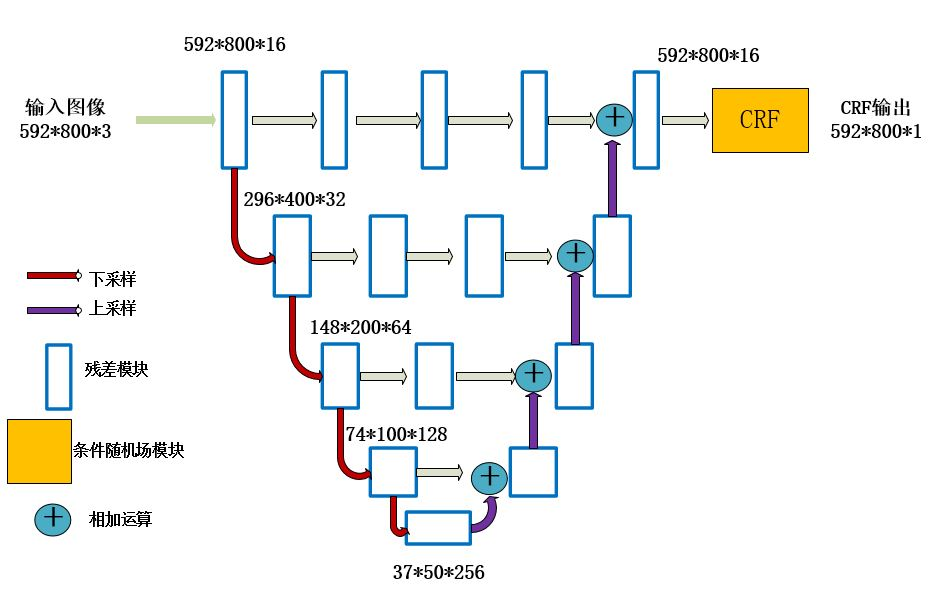
\includegraphics[width=13cm]{figure/chap5/arch.jpg}
	  \bicaption
		{分割网络架构图}
		{The Architecture of segmentation network}
	  \label{fig:chap5:arch}
	\end{figure}
	\begin{figure}[htb]
	  \centering
	  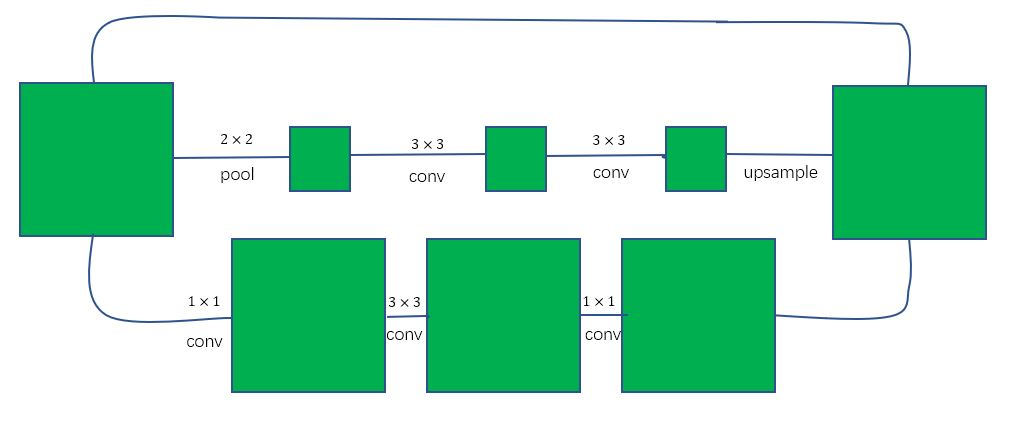
\includegraphics[width=11cm]{figure/chap4/residualpooling.jpg}
	  \bicaption
		{残差连接模块}
		{Residual connection module}
	  \label{fig:chap4:respool}
	\end{figure}
	
	残差网络\cite{he2016deep}能够在增加网络深度的同时使网络依然易于训练,更深的网络往往能够学习到
	更加抽象的特征从而提高网络的性能。因此本文使用了如图\ref{fig:chap4:respool}所示的残差连接模块\cite{chu2017multi}作为
	图\ref{fig:chap5:arch}中的基本连接单元,这种残差
	模块包含三个连接通路。中间的通路由于使用了降采样,在卷积核尺寸保持不变的情况下,输出神经元的感受野将扩大到原来的两倍。
	但由于使用了降采样,导致分辨率下降。但上下两条路径上包含高分辨率的信息。最后将这三个路径的输出叠加在一起作为残差
	连接模块的输出。这种连接方式在扩大网络的感受野的同时依然保持原来的分辨率。
	
\subsection{网络模型的训练}
	在线虫的实时跟踪任务中,神经网络模型的复杂度和实时性是需要关注的重点。太复杂的网络其推断时间耗时太长往往达不到
	实时性的要求,因此必须要在网络结构的设计时加以考虑,而网络训练和推断所消耗时间的评估依赖于所采用的机器学习库
	和网络模型运行的硬件平台。因此为了评估不同网络模型的复杂度和实时性,表\ref{tab:hardwareconfig}
	列出了本文中所有网络模型运行的软硬件平台。
	\begin{table}[!hpb]
	\centering
	\bicaption
    {算法运行的实验平台}
    {Experimental platform for algorithm running}
	\label{tab:hardwareconfig}
	\begin{tabular}{p{80pt}p{100pt}}
	\toprule
	平台参数 & 配置 \\
	\midrule
	操作系统 & Windows 10 家庭版\\
	系统内存 & 8g \\
	CPU & i5-6300HQ \\
	GPU & GTX 950M \\
	显存 & 4g \\
	深度学习库 & Tensorflow \\
	\bottomrule
	\end{tabular}
	\end{table}
	
	增强训练数据的多样性能够有效提高网络的泛化性能,特别是在较小的数据集上网络可能会出现过拟合的情况。为了
	提高网络的泛化能力,在网络训练阶段本文对训练集进行了数据增强。本文首先对训练图片以一定概率随机地进行水平镜像翻转或
	垂直镜像翻转,并将对应的标签做相同的变换。最后将训练图片加入一定量的高斯白噪声,以提高数据的多样性。
	在batchsize参数的选择上,考虑到本文训练图片的分辨率较高(为$592\times800\times3$)以及
	网络训练采用的硬件GPU显存较小(4g),因此不能将batchsize设置过大,本文这里将batchsize设为1,即采用单样本
	更新的方式训练网络。假设网络的最后一层输出是一张概率图设为$\Phi$,$y$为标签图(只包含0和1)。
	公式\ref{eq:loss}表示网络训练的交叉熵损失,通过随机梯度下降的方式不断地调整网络的模型参数使交叉熵损失不断下降。
	最终网络收敛到局部极小值或者全局最小值,训练损失将不会再下降。图\ref{fig:train_progress}表示训练过程中,训练
	损失和像素准确率随迭代次数的变化。图中可以看出随着迭代次数的增加,训练损失不断减小,像素准确率不断增加。网络在第
	1000次迭代后,网络基本已经收敛。经测试线虫前景轮廓分割网络推断单张图片的速度为16ms。
	\begin{equation}
		entropy\_loss = \sum_{i,j}y_{ij}\log \Phi_{ij} + (1-y_{ij})\log (1-\Phi_{ij}) \label{eq:loss}
	\end{equation}
	
	\begin{figure}[!htp]    
	\begin{minipage}[t]{0.5\linewidth}%设定图片下字的宽度,在此基础尽量满足图片的长宽    
		\centering    
		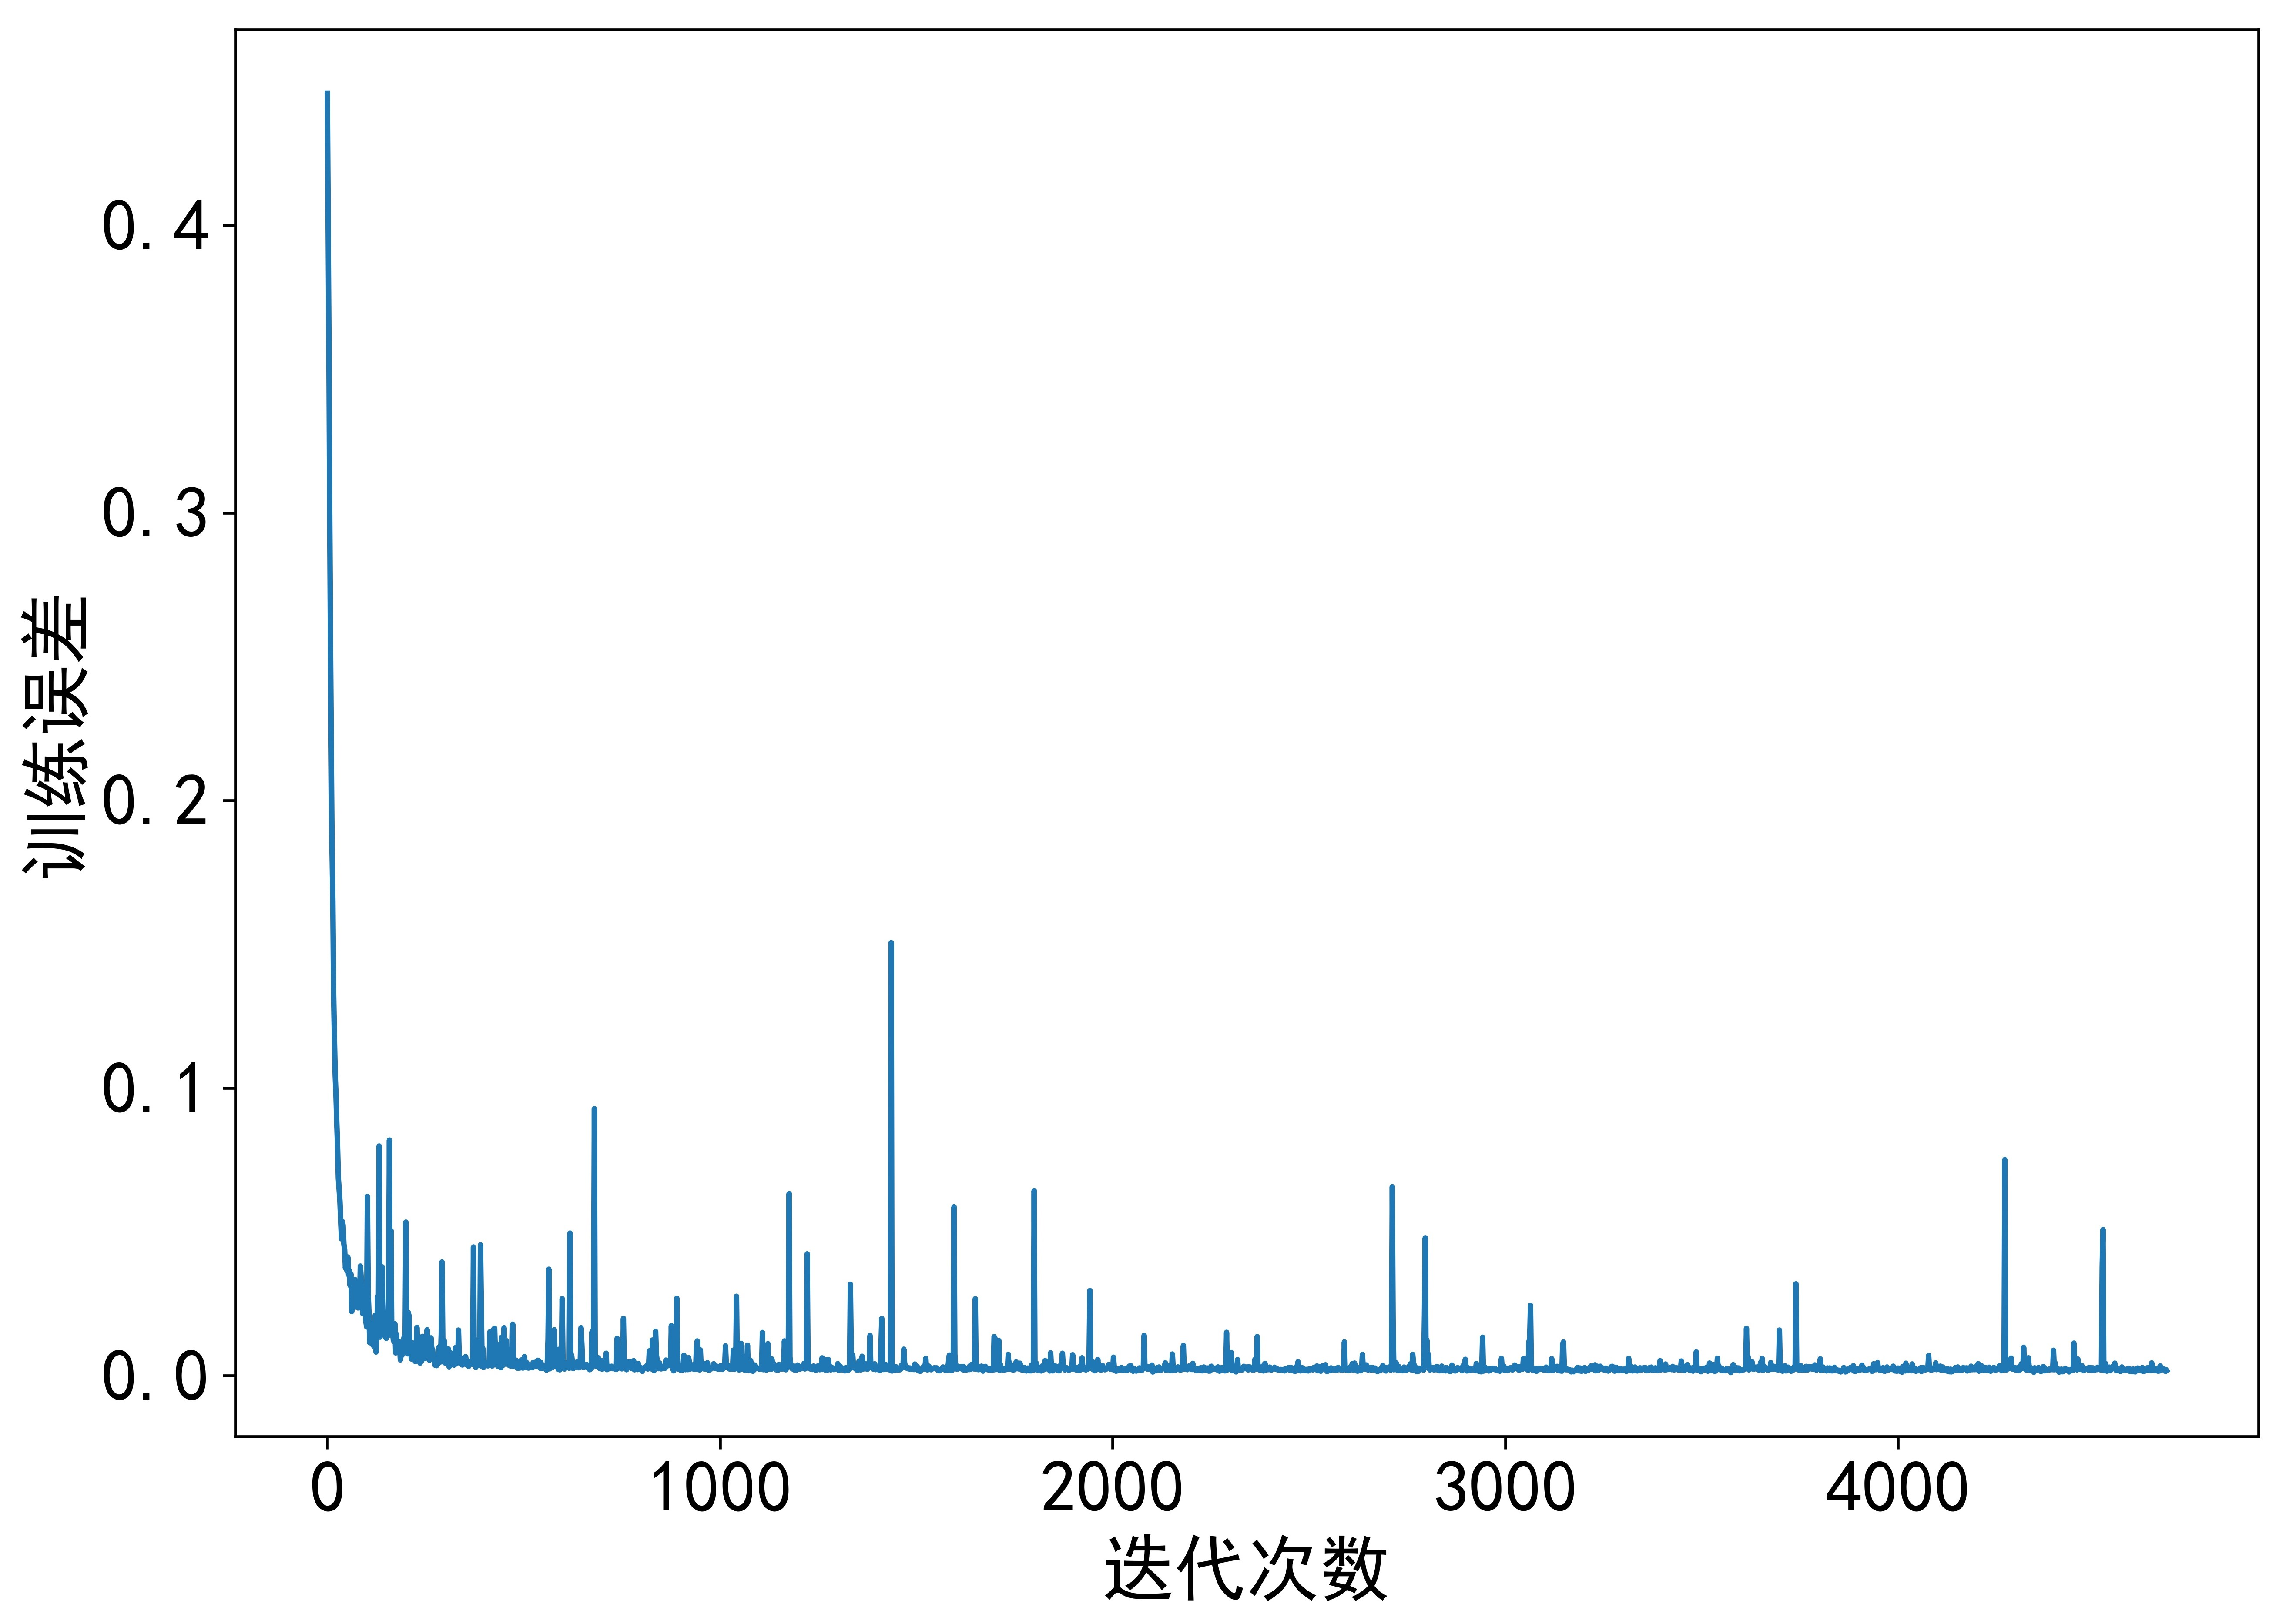
\includegraphics[width=1\linewidth]{figure/chap3/loss.jpg}    
		\caption*{(a) 训练损失随迭代次数的变化}%加*可以去掉默认前缀,作为图片单独的说明    
		\label{fig:angle}    
	\end{minipage}    
	\begin{minipage}[t]{0.5\linewidth}%需要几张添加即可,注意设定合适的linewidth    
		\centering    
		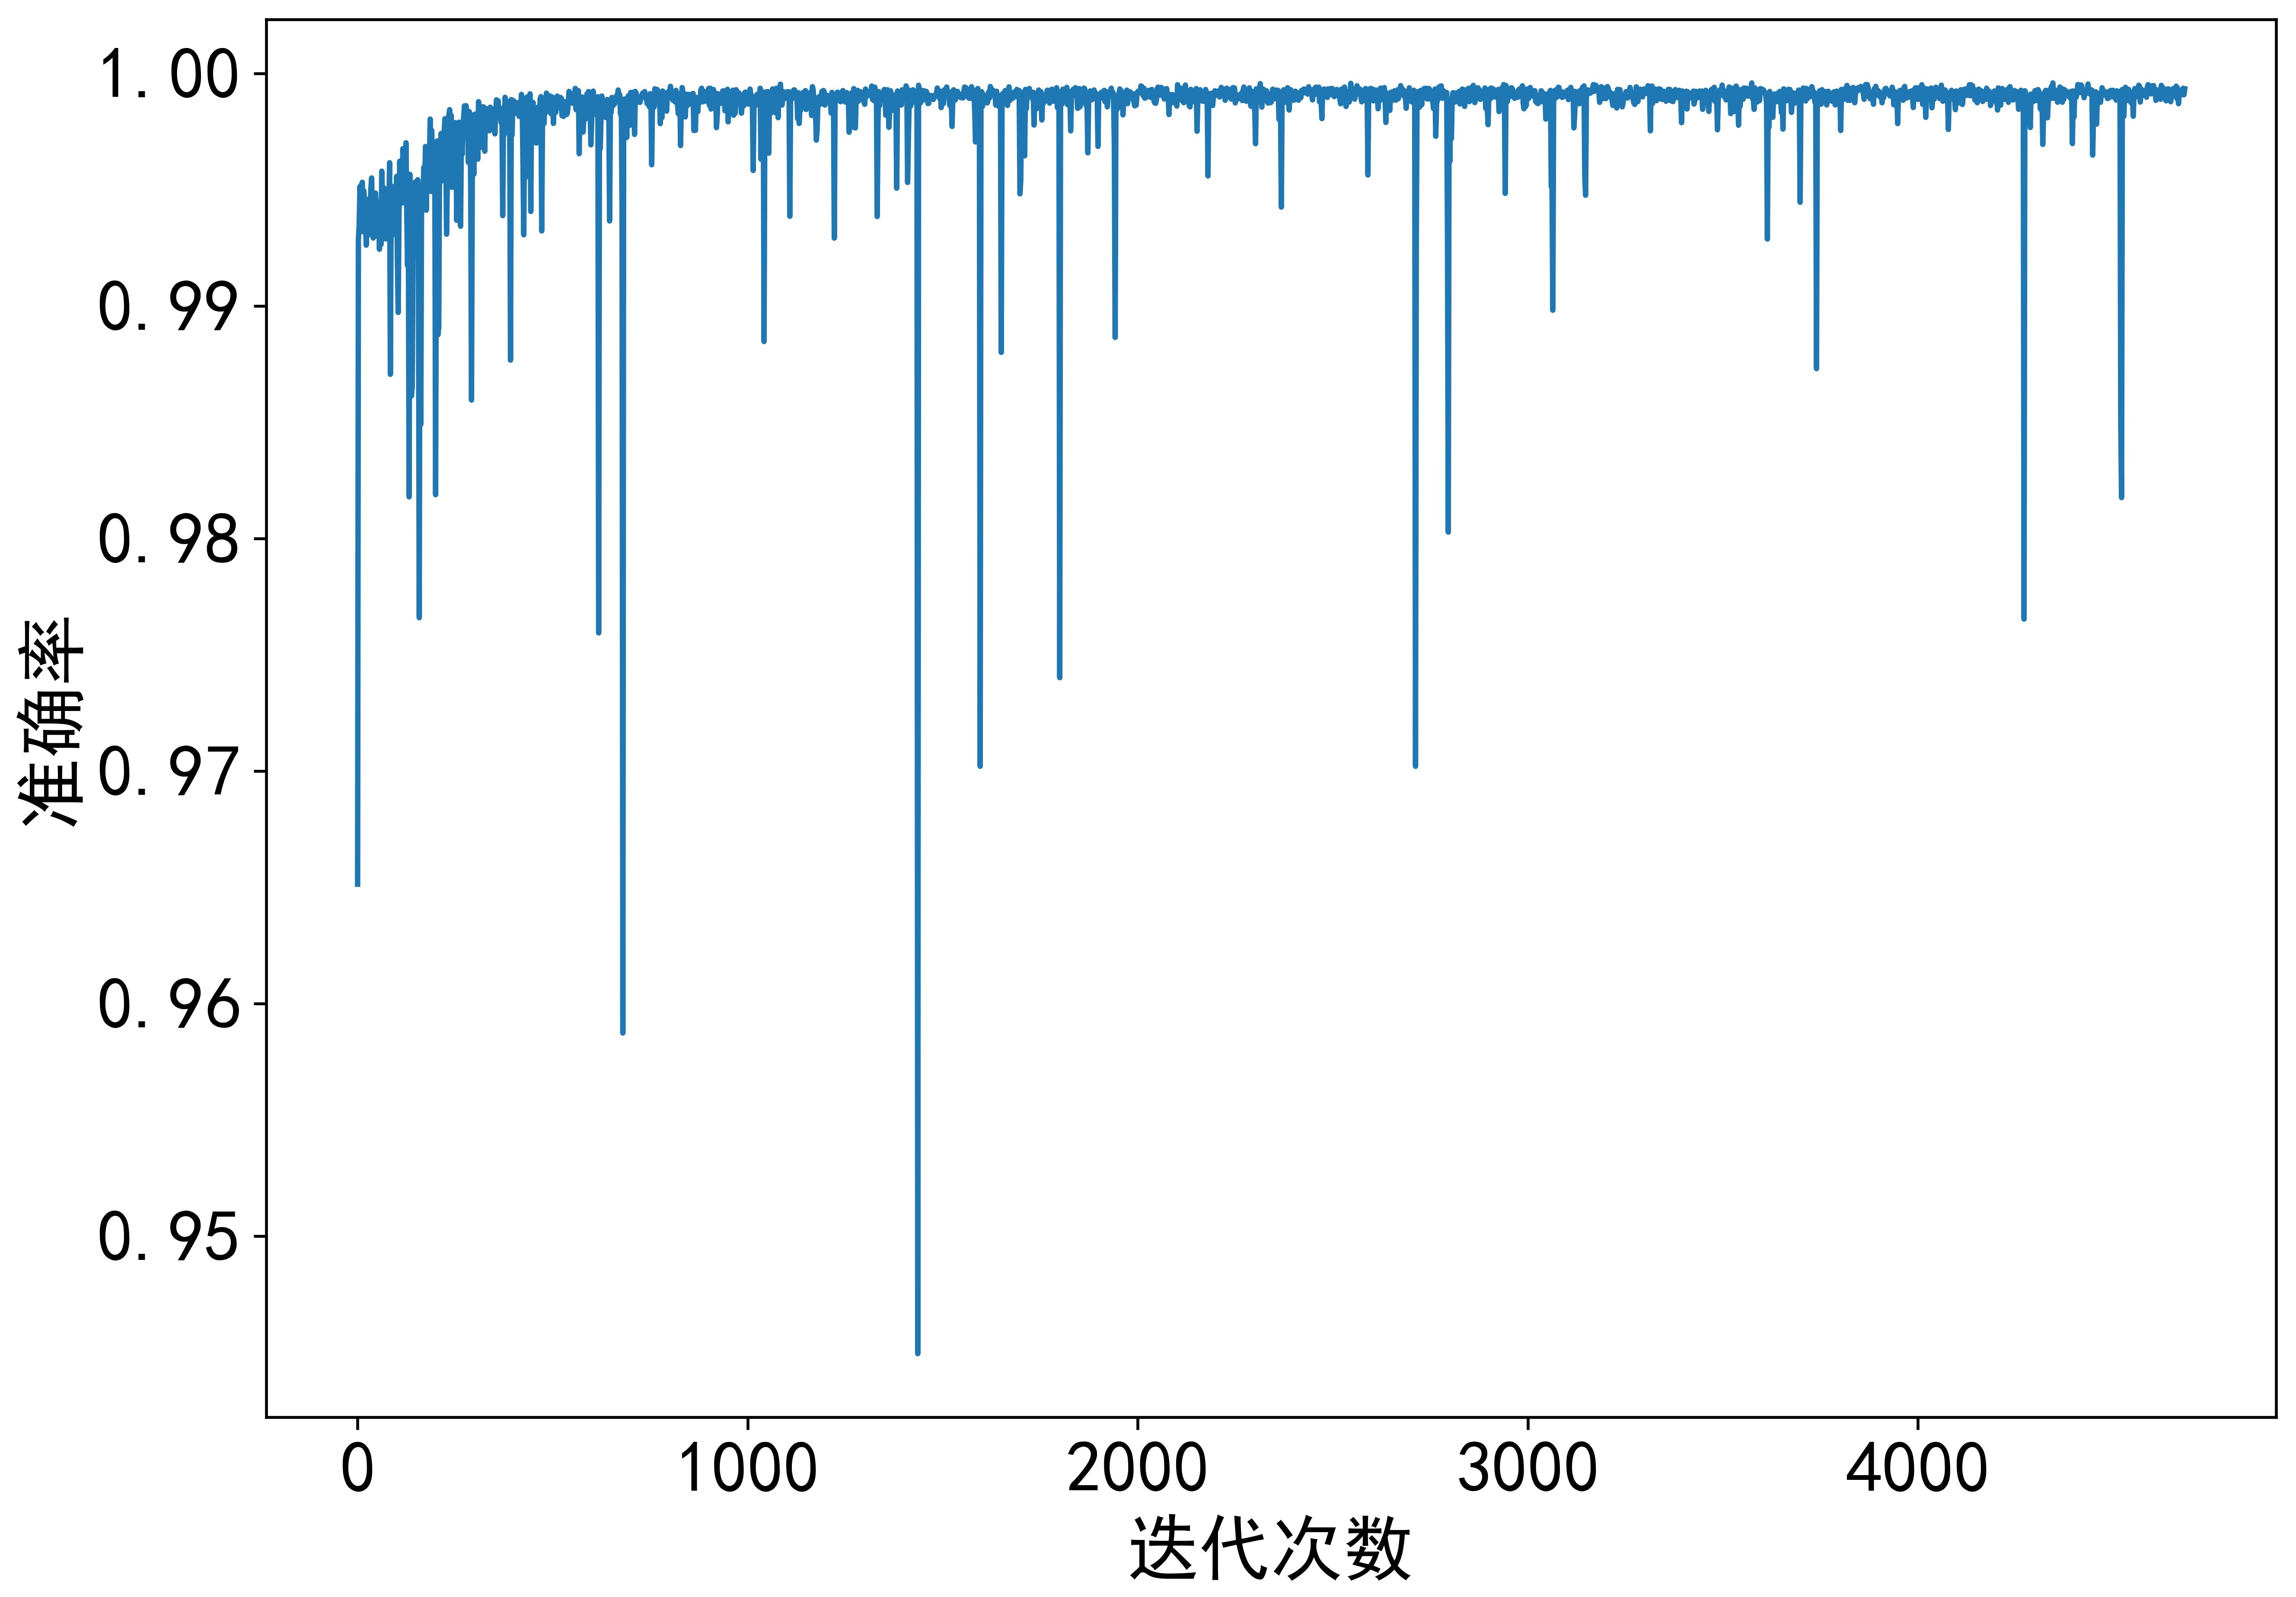
\includegraphics[width=1\linewidth]{figure/chap3/acc.jpg}    
		\caption*{(b) 像素准确率随迭代次数的变化}
		\label{fig:freq}
	\end{minipage}
	\bicaption{训练损失和像素准确率随迭代次数的变化}
	{Training loss and pixel accuracy varied with the number of iterations}%n张图片共享的说明
	\label{fig:train_progress}
	\end{figure}
\subsection{实验结果分析}
\subsubsection{评价指标}
	为了评估线虫前景轮廓分割网络的分割性能,需要一些量化指标来量化分割的结果。本文采用的三个
	量化指标分别为:过分割率(Over Segmentation, OR)、欠分割率(Under Segmentation, UR)以及总体
	分割误差率(Overall Error Rate, ER)\cite{Liu2006Set}。分别由公式\ref{eq:OR}、\ref{eq:UR}和\ref{eq:ER}计算。
	其中$Q_p$表示目标像素被误分类为背景像素的数目,$U_p$为背景像素被误分类为目标像素的数目,$D_n$表示背景像素点
	的数目,$D_p$表示目标像素点的数目。
		\begin{equation}
		OR = Q_p/D_p \label{eq:OR}
		\end{equation}
		\begin{equation}
		UR = U_p/D_n \label{eq:UR}
		\end{equation}
		\begin{equation}
		ER = (Q_p+U_p)/(D_p+D_n)\label{eq:ER}
		\end{equation}
\subsubsection{分割效果对比}
	为了比较分析不同算法的前景轮廓分割效果,本小节我们将本章提出的基于条件随机场的卷积分割算法与传统的
	前景轮廓提取方法进行了对比。图\ref{fig:comp_res}显示了不同算法的分割结果,
	从图中可以看出基于模糊C均值聚类的
	分割方法\cite{peizhuang1983pattern}和基于阈值分割的OTSU算法\cite{otsu1979threshold}的分割结果
	存在大量的像素分类错误。从图\ref{fig:comp_res}a可以看出,图像底部微流控芯片结构
	部分的亮度较高,但这部分区域的像素应该属于背景像素,这两种基于像素的分割方法都将这些区域分类为前景像素。另一方面,从原图可以看出线虫的轮廓中心处的
	亮度较低,这两种算法都将这些区域的像素分类为背景,造成了线虫轮廓的不连续以及存在孔洞。虽然经过后处理步骤
	可以针对单张图像过滤掉非线虫轮廓,以及运用形态学图像处理技术可以消除掉线虫轮廓中的空洞和不连续等缺陷。但在
	线虫视频的自动化分析任务中,由于每一帧图像的噪声情况都不一样,因此很难确定一个全局的阈值。 基于高斯混合模型的
	背景减除方法\cite{zivkovic2006efficient}虽然比基
	于阈值的分割方法和基于聚类的分割方法分割结果有很大的改善,但线虫的轮廓依然存在不连续的
	情况。基于背景减除的分割方法最大的不足在于其只能针对背景固定的视频,因此这种分割方法具有很大的局限性。
	图\ref{fig:comp_res}f是本文不带条件随机场模块的卷积网络(去掉CRF模块,同时用$1\times1$的卷积将特征的
	通道数变为1作为网络的输出)分割的结果。
	从图中可以看出去掉CRF模块后,卷积分割网络由于没有考虑到空间中相邻像素的相关性,从而导致线虫轮廓的不连续,
	分割性能较差。而条件随机场模块能够显著地改善线虫前景轮廓分割中的不连续等情况,与以上的方法相比,其分割性能
	要优于其他的方法且不依赖于超参数的选择,具有很好的鲁棒性。
	
\begin{figure}[!htp]
	  \centering

	  \begin{subfigure}{\linewidth}
		\centering
		\begin{minipage}[b]{\linewidth}
		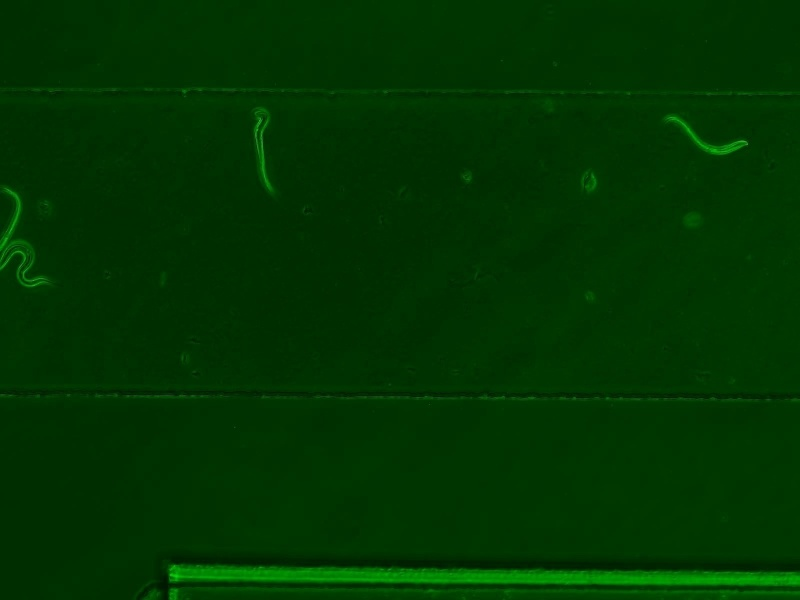
\includegraphics[width=0.33\linewidth,natwidth=800,natheight=600]{figure/chap3/img/441.orgin.851.jpg}
		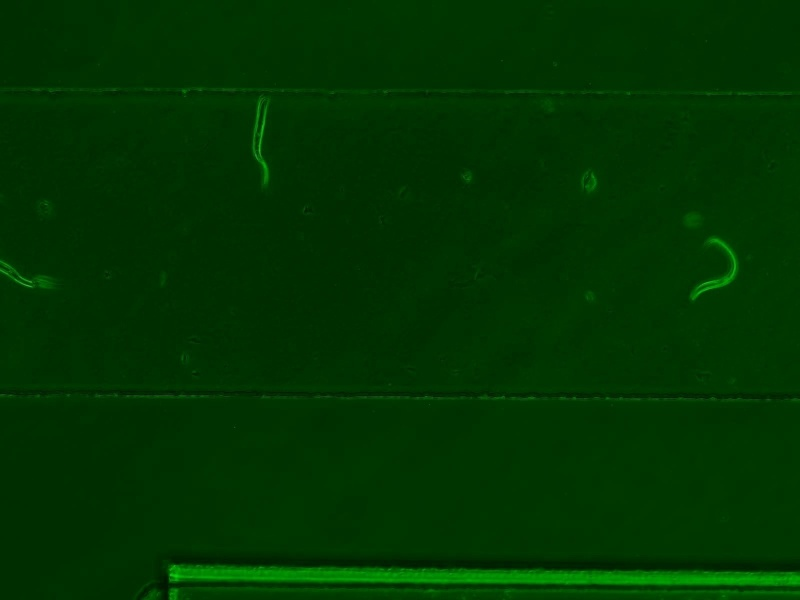
\includegraphics[width=0.33\linewidth,natwidth=800,natheight=600]{figure/chap3/img/441.orgin.1051.jpg}
		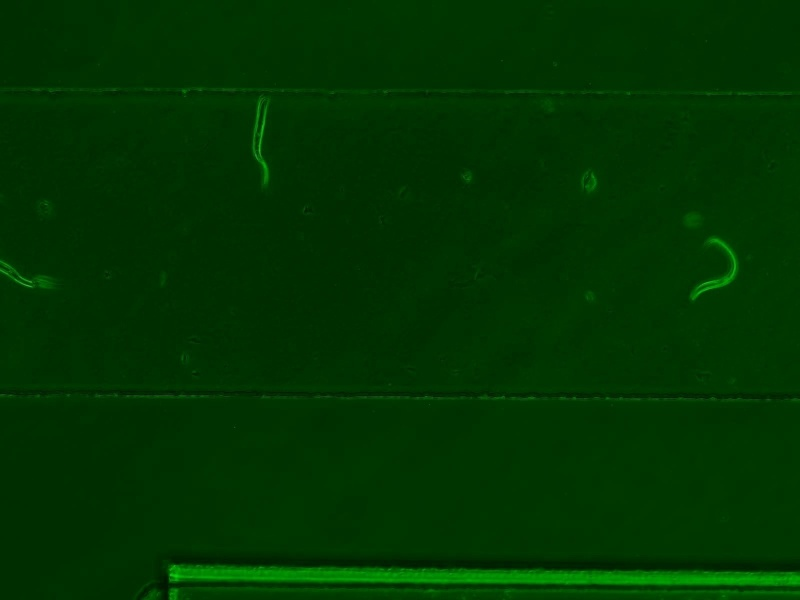
\includegraphics[width=0.33\linewidth,natwidth=800,natheight=600]{figure/chap3/img/441.orgin.1051.jpg}
		\end{minipage}
		\caption{线虫原图像}
	  \end{subfigure}

	 \begin{subfigure}{\linewidth}
		\centering
		\begin{minipage}[b]{\linewidth}
		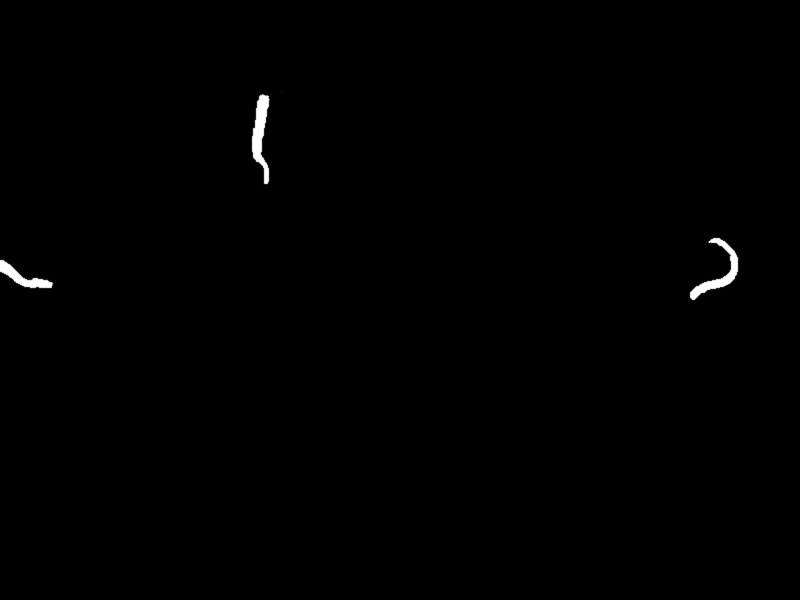
\includegraphics[width=0.33\linewidth,natwidth=800,natheight=600]{figure/chap3/label/441.orgin.1051.jpg}
		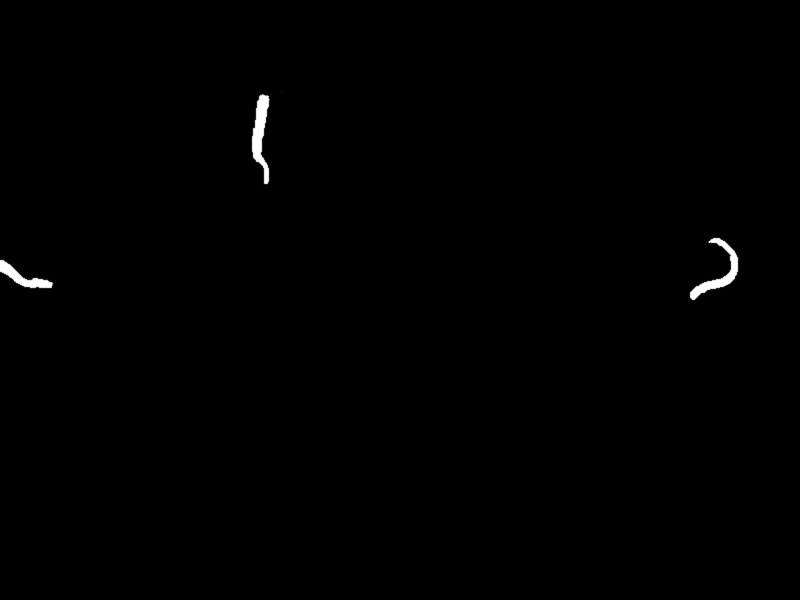
\includegraphics[width=0.33\linewidth,natwidth=800,natheight=600]{figure/chap3/label/441.orgin.1051.jpg}
		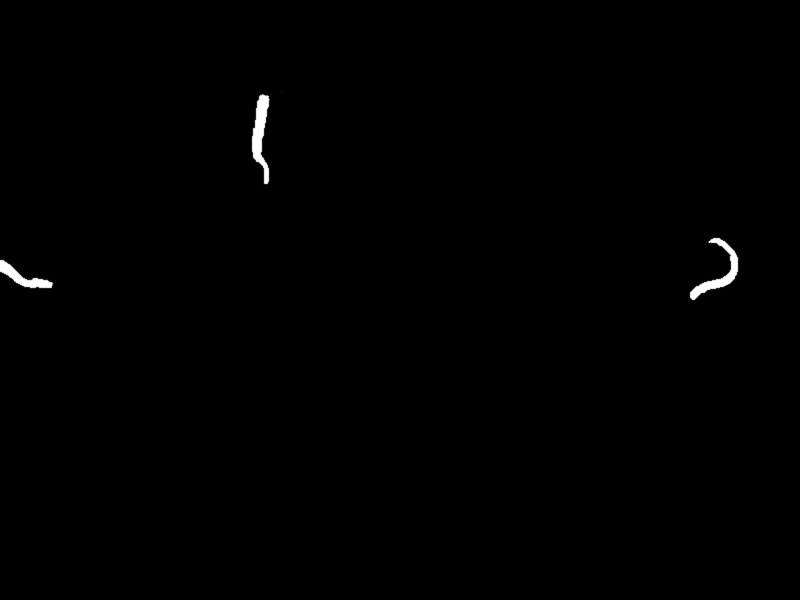
\includegraphics[width=0.33\linewidth,natwidth=800,natheight=600]{figure/chap3/label/441.orgin.1051.jpg}
		\end{minipage}
		\caption{分割标签}
	  \end{subfigure}

	 \begin{subfigure}{\linewidth}
		\centering
		\begin{minipage}[b]{\linewidth}
		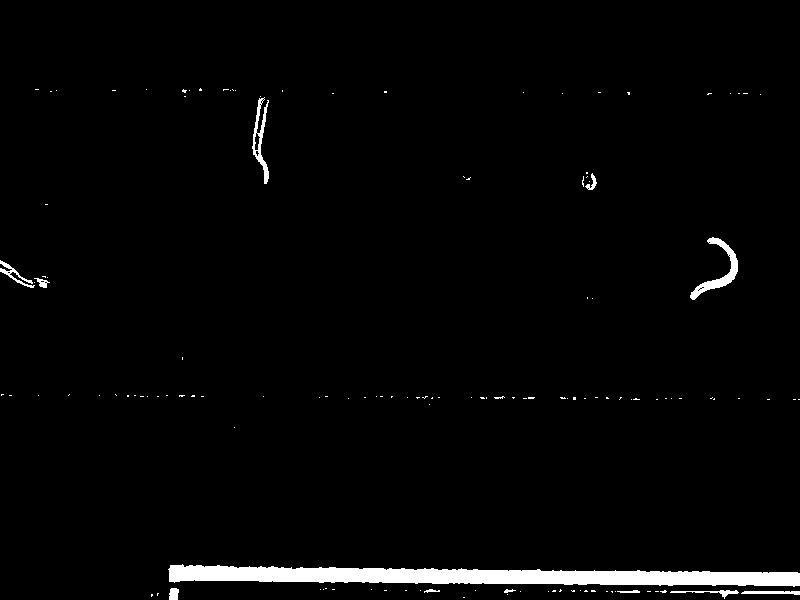
\includegraphics[width=0.33\linewidth,natwidth=800,natheight=600]{figure/chap3/test_otsu/441.orgin.1051.jpg}
		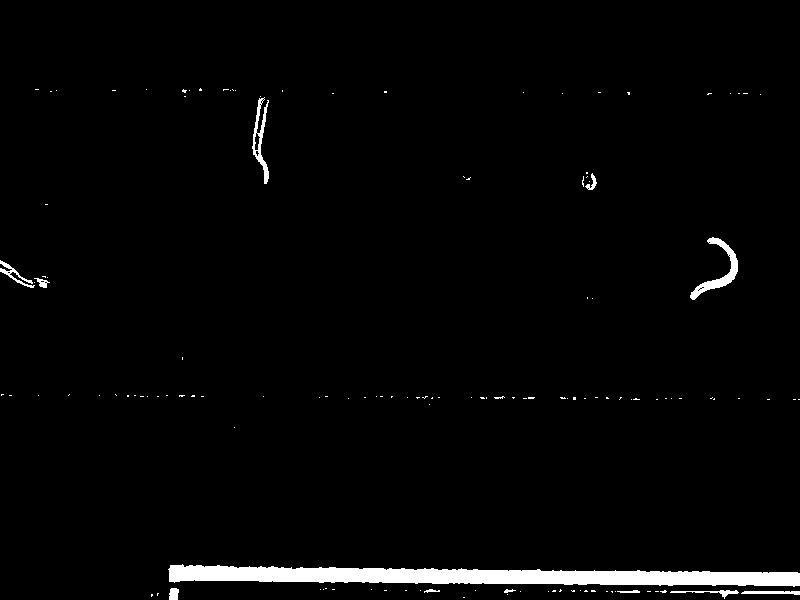
\includegraphics[width=0.33\linewidth,natwidth=800,natheight=600]{figure/chap3/test_otsu/441.orgin.1051.jpg}
		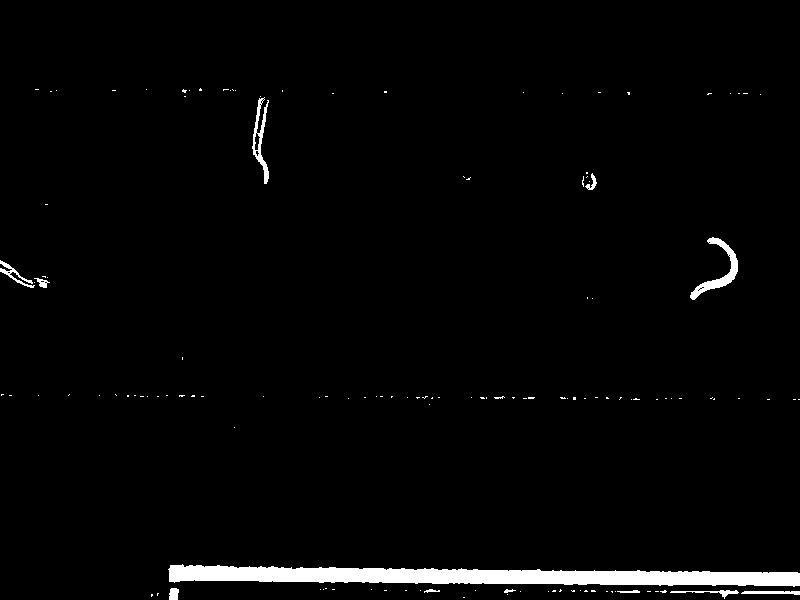
\includegraphics[width=0.33\linewidth,natwidth=800,natheight=600]{figure/chap3/test_otsu/441.orgin.1051.jpg}
		\end{minipage}
		\caption{OTSU阈值分割算法结果}
	  \end{subfigure}

	 \begin{subfigure}{\linewidth}
		\centering
		\begin{minipage}[b]{\linewidth}
		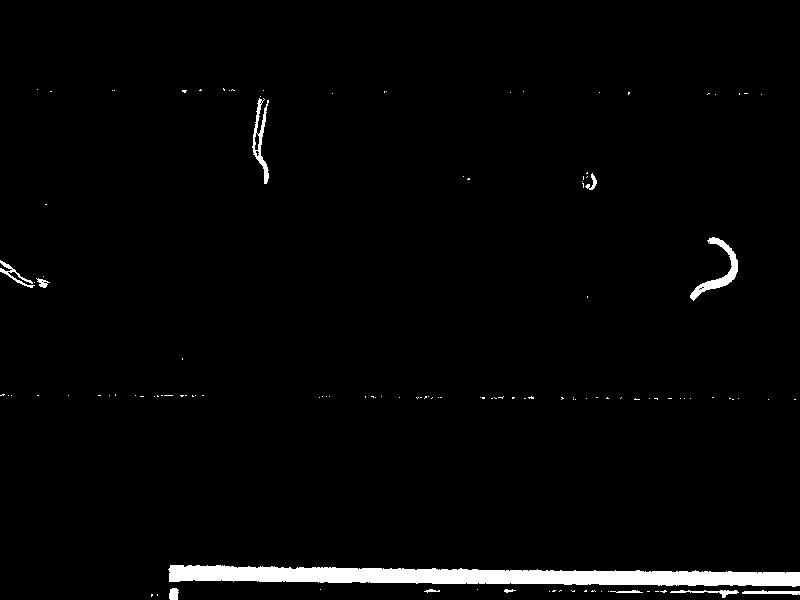
\includegraphics[width=0.33\linewidth,natwidth=800,natheight=600]{figure/chap3/test_fcm/441.orgin.1051.jpg}
		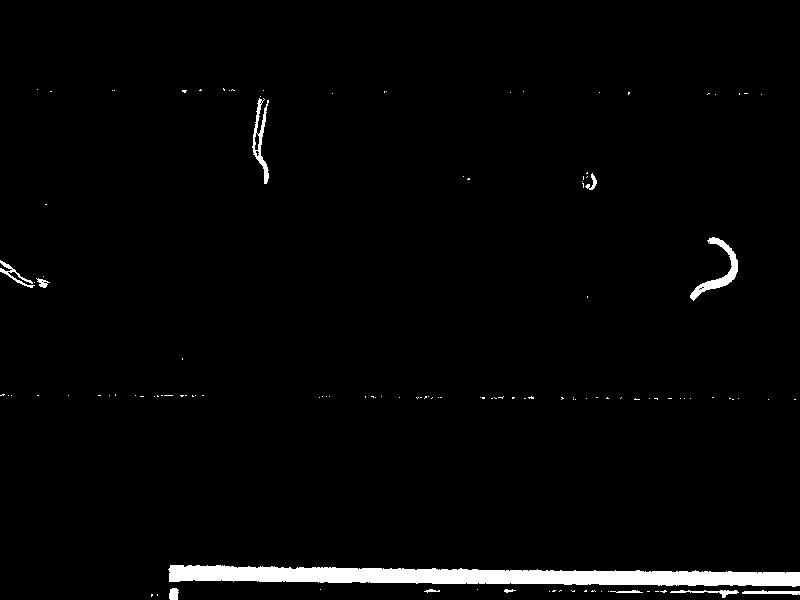
\includegraphics[width=0.33\linewidth,natwidth=800,natheight=600]{figure/chap3/test_fcm/441.orgin.1051.jpg}
		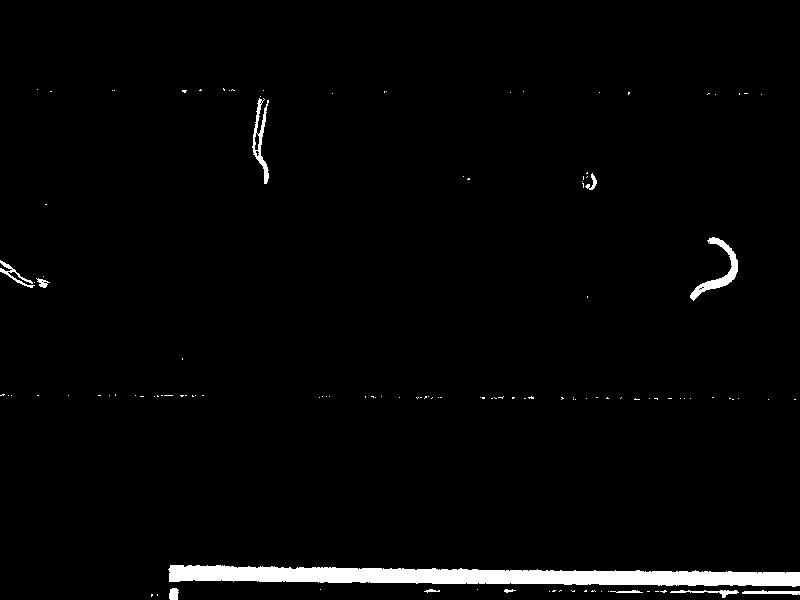
\includegraphics[width=0.33\linewidth,natwidth=800,natheight=600]{figure/chap3/test_fcm/441.orgin.1051.jpg}
		\end{minipage}
		\caption{模糊C均值聚类算法分割结果}
	  \end{subfigure}

	  \begin{subfigure}{\linewidth}
		\centering
		\begin{minipage}[b]{\linewidth}
		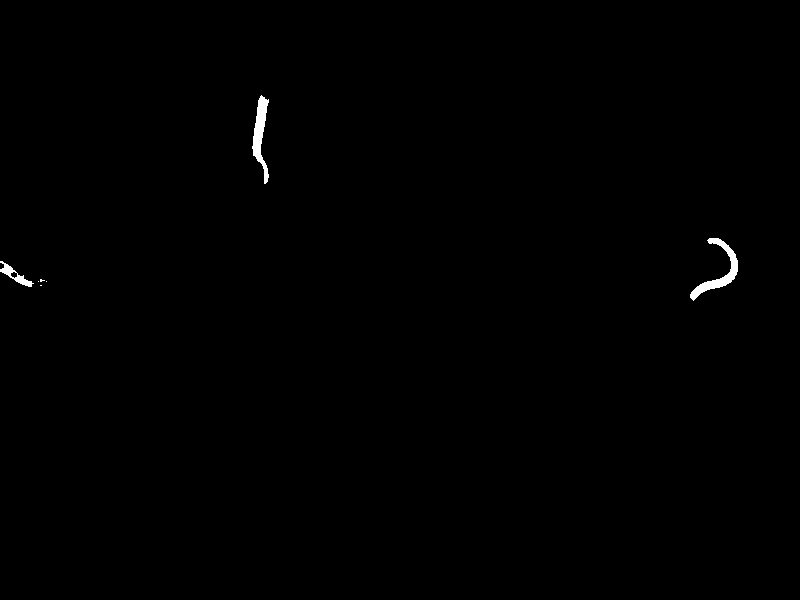
\includegraphics[width=0.33\linewidth,natwidth=800,natheight=600]{figure/chap3/test_bksub/441.orgin.1051.jpg}
		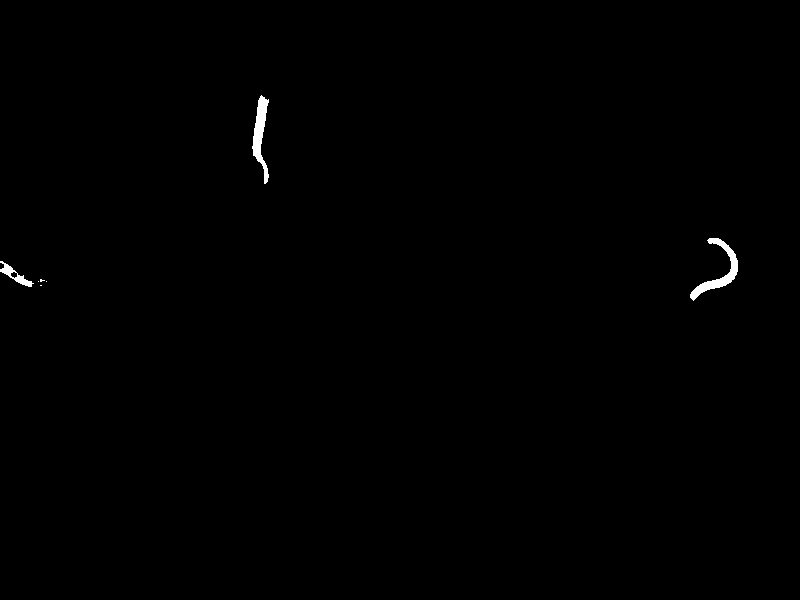
\includegraphics[width=0.33\linewidth,natwidth=800,natheight=600]{figure/chap3/test_bksub/441.orgin.1051.jpg}
		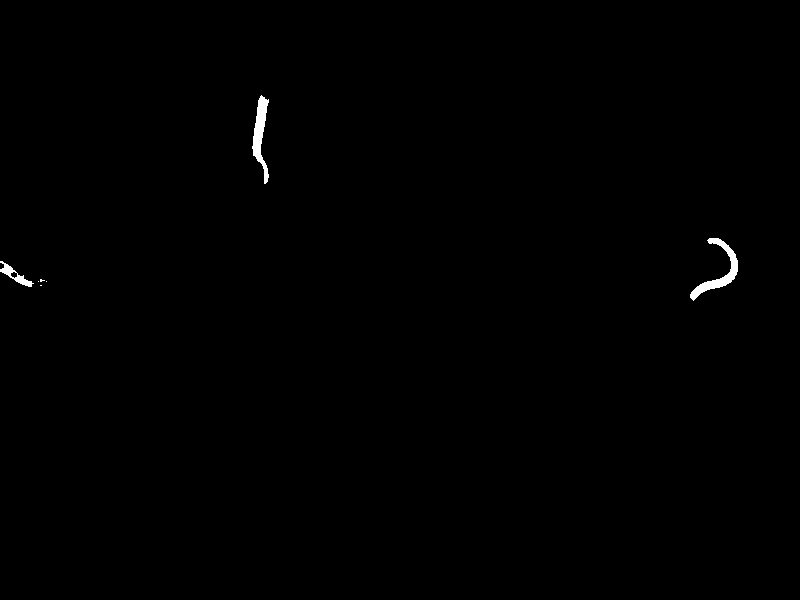
\includegraphics[width=0.33\linewidth,natwidth=800,natheight=600]{figure/chap3/test_bksub/441.orgin.1051.jpg}
		\end{minipage}
		\caption*{(e)混合高斯背景建模的分割算法结果}
	  \end{subfigure}
\end{figure}
\begin{figure}[!htp]
	\addtocounter{subfigure}{5}
		\centering
		\ContinuedFloat
	  \begin{subfigure}{\linewidth}
		\centering
		\begin{minipage}[b]{\linewidth}
		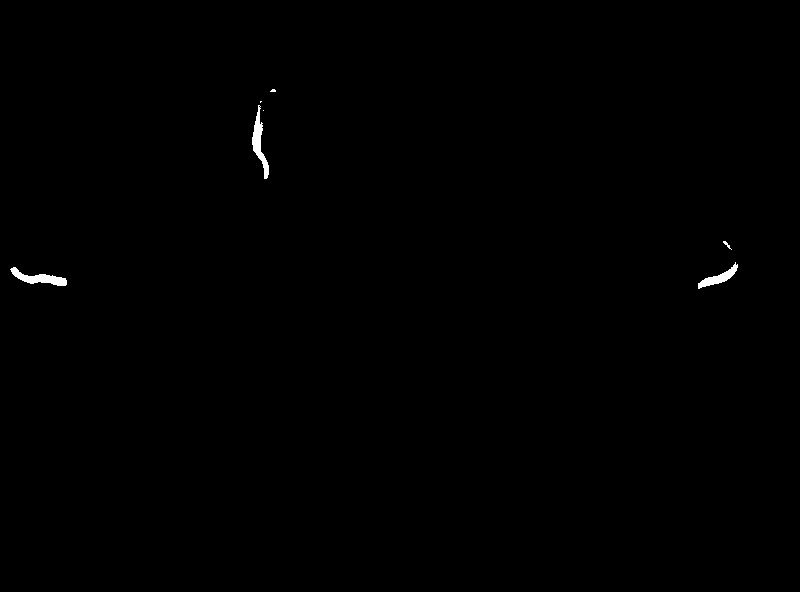
\includegraphics[width=0.33\linewidth,natwidth=800,natheight=600]{figure/chap3/test2/441.orgin.1051.jpg}
		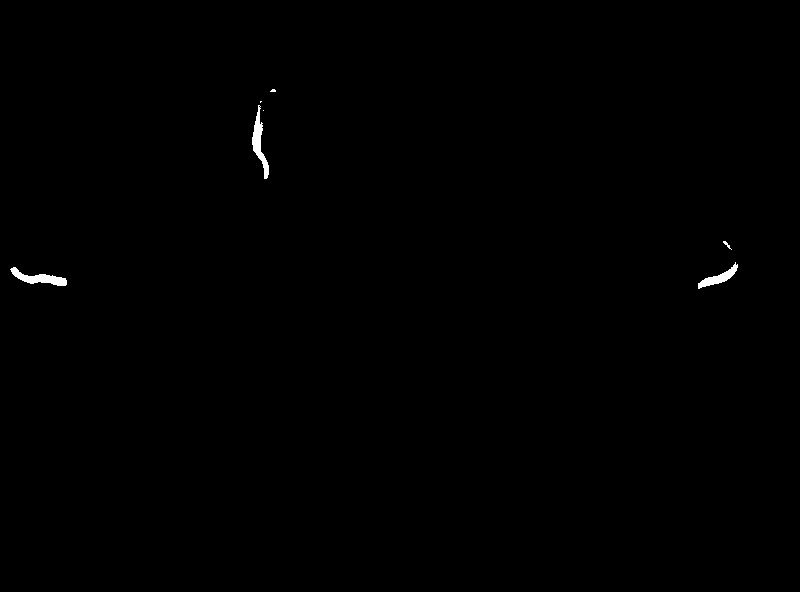
\includegraphics[width=0.33\linewidth,natwidth=800,natheight=600]{figure/chap3/test2/441.orgin.1051.jpg}
		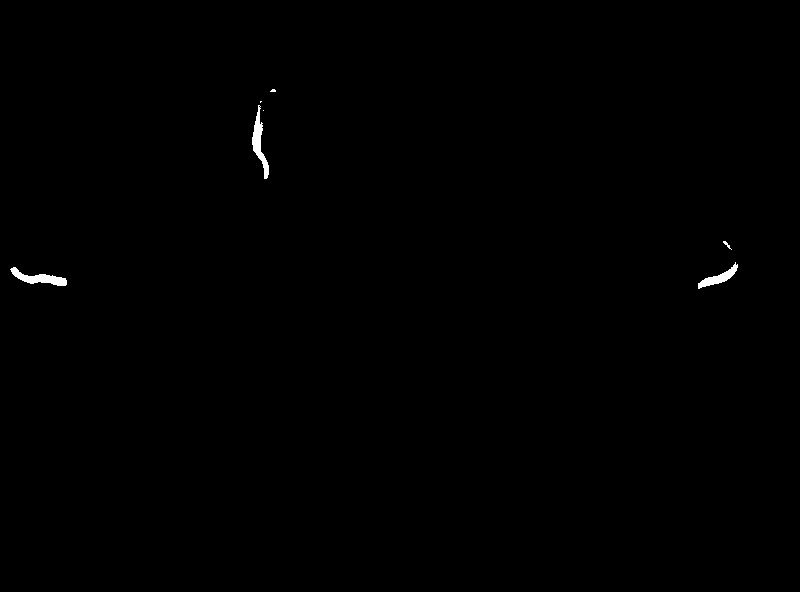
\includegraphics[width=0.33\linewidth,natwidth=800,natheight=600]{figure/chap3/test2/441.orgin.1051.jpg}
		\end{minipage}
		\caption*{(f)本文算法分割结果(没有条件随机场模块)}
	  \end{subfigure}

	  \begin{subfigure}{\linewidth}
		\centering
		\begin{minipage}[b]{\linewidth}
		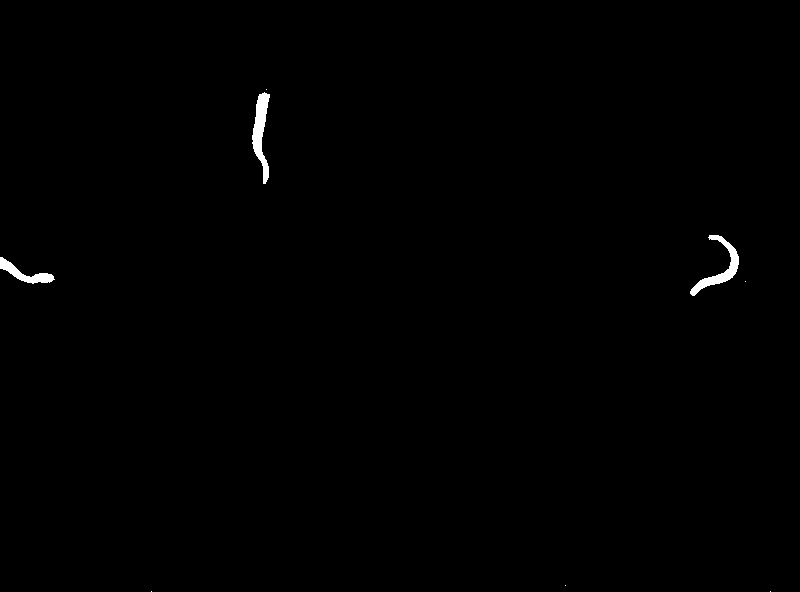
\includegraphics[width=0.33\linewidth,natwidth=800,natheight=600]{figure/chap3/test1/441.orgin.1051.jpg}
		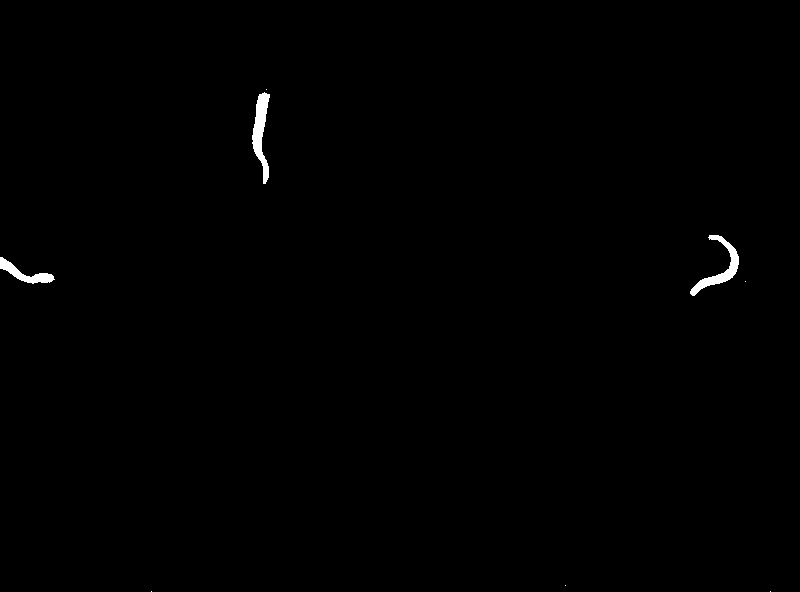
\includegraphics[width=0.33\linewidth,natwidth=800,natheight=600]{figure/chap3/test1/441.orgin.1051.jpg}
		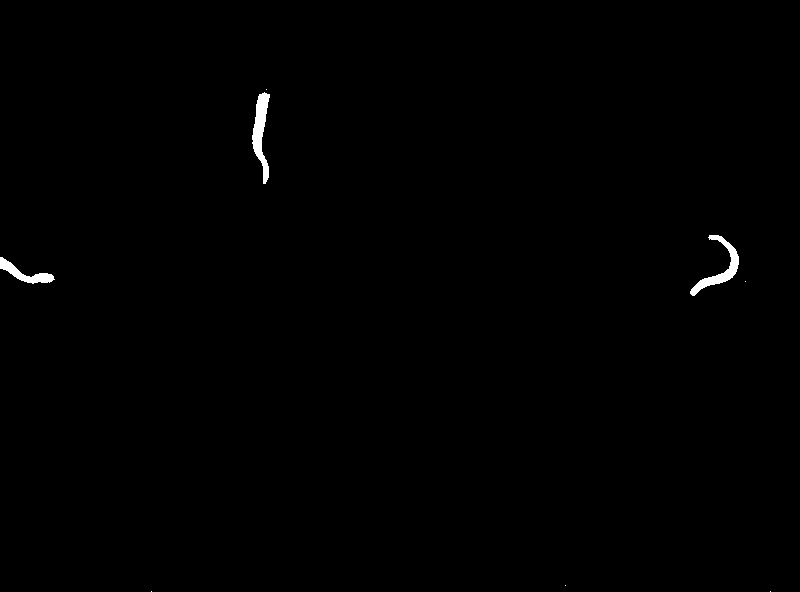
\includegraphics[width=0.33\linewidth,natwidth=800,natheight=600]{figure/chap3/test1/441.orgin.1051.jpg}
		\end{minipage}
		\caption*{(g)本文算法分割结果}
	  \end{subfigure}
	  \bicaption{不同分割算法的分割结果}{The result of different segmentation methods}
	  \label{fig:comp_res}
\end{figure}
\subsubsection{分割性能的量化分析}
	\begin{table}[htbp]
	\centering
	\bicaption
    {不同分割方法的性能比较}
    {Performance comparison of different segmentation methods}
	\label{tab:metrics}
	\begin{tabular}{>{\centering}p{100pt}>{\raggedleft\arraybackslash}p{60pt}>{\raggedleft\arraybackslash}p{60pt}>{\raggedleft\arraybackslash}p{60pt}}
	\toprule
	算法&过分割率&欠分割率&总体误差\\
	\midrule
	本文算法 &12.29\% &0.01\% & 0.11\% \\
	本文算法(无CRF模块)&26.93\% & 0.03\% &0.17\% \\
	背景减除  &19.55\% & 0.02\%& 0.12\% \\
	OTSU算法 &26.62\% & 2.12\% & 2.25\% \\
	FCM 算法 &27.41\% & 2.15\% & 2.28\% \\
	\bottomrule
	\end{tabular}
	\end{table}
	为了定量地分析不同分割算法的性能,本文采用了三种性能指标对不同分割算法在测试集上分割的结果进行量化,结果如表\ref{tab:metrics}所示。
	从表中可以看出基于阈值分割的OTSU算法和基于聚类的FCM算法在过分割率、欠分割率以及总体误差三个指标上均表现较差。
	另外,没有使用CRF的卷积分割网络在三个指标上的表现均弱于基于背景减除的分割方法。但在卷积网络后端加入CRF模块后,网络的分割性能
	有了很大的提升,其分割性能要优于其他的分割算法,总体的像素误差下降到$0.11\%$。
\section{基于深度卷积网络的线虫轮廓解析}
	多线虫跟踪问题中,多线虫轮廓之间相互纠缠是造成线虫跟踪丢失的主要原因,是实现单个线虫长期跟踪的关键。
	如图\ref{fig:multi-worms}所示,是一张经过线虫前景轮廓分割后得到的二值化图像,
	图中线虫轮廓之间出现严重的相互遮挡的情况,多个单线虫轮廓融合为一个连通域
	。虽然人眼可以很轻松地辨别出图中所有单个线虫的轮廓,但自动化地解析出单个线虫的轮廓却十分困难。尽管深度学习在图像分割任务中取得了很大的成功,
	但线虫轮廓的解析不同于图像分割,因此不能直接转为一个端到端的学习问题。
	Yurchenko等人\cite{yurchenko2017parsing}于2017年提出了一种线虫解析的算法,该算法首先在经过前景背景分割的
	二值化图像上随机选取许多的图像块,使其尽可能覆盖所有的线虫轮廓,并通过神经网络提取每一个图像块的特征向量。
	然后建立一个大的线虫姿势搜索库,库中包含大量的线虫姿势和与之对应的特征向量。将图像块对应的特征向量作为键值
	通过最近邻的方式在线虫姿势搜索库中搜索到最佳的匹配,从而得到线虫的姿势估计。最后通过整数规划的方式去除掉
	重复的线虫轮廓,从而得到线虫解析的结果。该算法的不足在于,为了使这个库能够包含各种大小和姿势的线虫
	,需要建立一个非常大的搜索库(大约4百万)。库的规模限制了轮廓解析的精度,所以只能得到近似的解析结果。另一面方面
	在一个很大的库中搜索匹配需要大量的时间,因此实时性是该算法的另一个不足。
	本文提出了一种基于深度卷积网络的线虫轮廓解析算法尝试解决这一问题,与以上提到的轮廓解析算法不同,本文提出的轮廓
	解析算法不需要建立搜索库,而是直接将图像块输入到网络,网络可以自动输出中央线虫的轮廓。由于神经网络模型在推断
	阶段速度很快,本文提出的线虫轮廓解析算法具有很好的实时性能。
	\begin{figure}[!htp]    
	\begin{minipage}[t]{0.49\linewidth}%设定图片下字的宽度,在此基础尽量满足图片的长宽    
		\centering    
		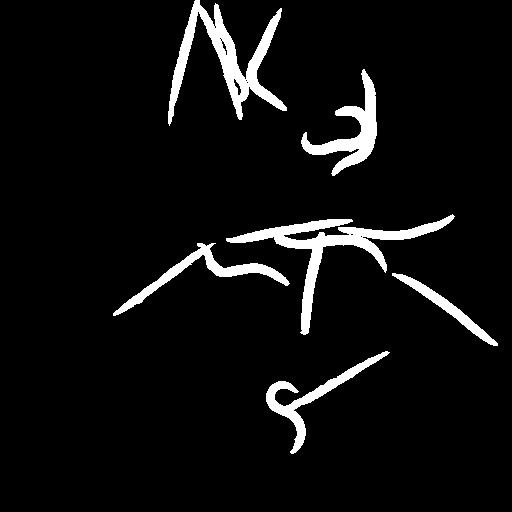
\includegraphics[width=1\linewidth]{figure/chap4/multi-worm.jpg}    
		%\caption*{(a) 训练损失随迭代次数的变化}%加*可以去掉默认前缀,作为图片单独的说明    
		\label{fig:angle}    
	\end{minipage}    
	\begin{minipage}[t]{0.49\linewidth}%需要几张添加即可,注意设定合适的linewidth    
		\centering    
		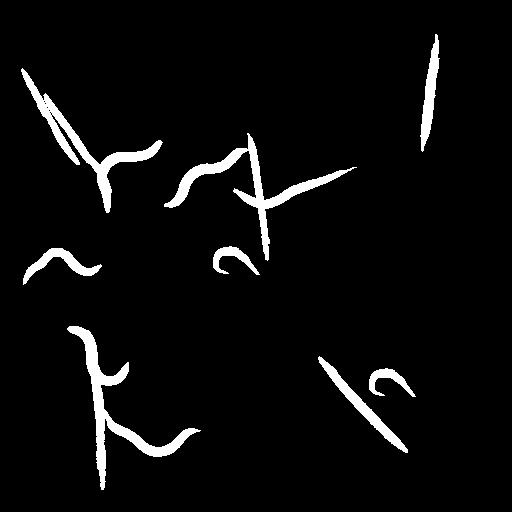
\includegraphics[width=1\linewidth]{figure/chap4/multi-worm1.jpg}    
		%\caption*{(b) 像素准确率随迭代次数的变化}
		\label{fig:freq}
	\end{minipage}
	\bicaption{多线虫轮廓相互纠缠示例}
	{Example of multi-worm entangled with each other}%Multi-lineworm contours entangled with each other
	\label{fig:multi-worms}
	\end{figure}
\subsection{线虫轮廓解析方法介绍}
	本文提出的线虫轮廓解析算法的关键在于设计了一个只对位于图片中央的线虫轮廓敏感的神经网络,而对非图片中央位置的线虫轮廓不敏感。当输入
	一幅包含多线虫轮廓的前景图像时,网络的输出为中央线虫轮廓的图像。
	形式化的描述如下:假设一幅图片中包含$N+1$个线虫轮廓,定义一个集合$E =\{e_0,e_1,\dots,e_N\}$,其中$e_0$表示轮廓位于图片
	中央的线虫,$e_i$包含线虫重心坐标、轮廓以及方向等信息。$I(E)=R(\{e_0,e_1,\dots,e_N\};\xi)$表示由集合E渲染得到的包含$N+1$个线虫的图片,R表示
	渲染函数,$\xi$表示随机噪声。$I(E_0)=R(\{e_0\};\xi)$表示由中间线虫渲染得到的图片。我们希望得到这样的映射
	$S:I(E)\rightarrow I(E_0)$,映射函数$S$通过一个深度卷积网络加以实现,本文将其命名为SingleOut-net网络。
	\begin{figure}[!htp]
    \centering
    \begin{tikzpicture}[node distance=2.5cm,auto]
	\tikzstyle{process} = [rectangle,rounded corners,very thick,minimum width = 3cm,text width=3cm,
	inner sep=2pt,minimum height =2cm, text centered, draw = black]
    \node (init) [process] {在待解析图像的前景区域产生随机点};
    \node (allocate) [process, right of=init,node distance=4cm] {以随机点为中心获取固定尺寸的图像块};
    \node (open) [process, right of=allocate,node distance=4cm] {SingleOut-Net输出中央线虫轮廓};
    \node (op) [process, below of=open,yshift=0.5cm,node distance=4cm] {输出结果后处理};
    \node (close) [process, left of=op,node distance=4cm] {滤除重复的线虫轮廓};
	\node (free) [process, left of=close,node distance=4cm] {得到最终的解析结果};
    %连接具体形状
    \draw [arrow](init) -- (allocate);
    \draw [arrow](allocate) -- (open);
    \draw [arrow](open) -- (op);
    \draw [arrow](op) -- (close);
	\draw [arrow](close) -- (free);
	\end{tikzpicture}
    \bicaption{线虫轮廓解析的算法流程}
	{Algorithm flow for C.elegans image parser}
    \label{fig:chap4:flow}
	\end{figure}
	
	如图\ref{fig:chap4:flow}是本文提出的线虫轮廓解析方法的主要流程。首先假定已经从前景轮廓分割的步骤中已经得到
	包含多线虫轮廓的二值化图像如图\ref{fig:multi-worms}所示,轮廓解析算法的第一步是在该二值化图像的前景像素中(即非零值像素)产生足够多的随机点使得每个线虫轮廓上至少
	包含一个随机点。然后以这些随机像素点为中心在原图中获取固定尺寸的图像块,将这些图像块输入到训练好的SingleOut-Net
	网络,网络输出为图像块中央位置的线虫轮廓图像。对SingleOut-Net输出的图像进行简单的后处理及二值化操作,
	然后运用轮廓提取算法即可得到这些图像块中央位置线虫的轮廓。由于在随机点产生阶段,同一个线虫轮廓可能包含不止一个随机点。因此由SingleOut-Net网络输出
	的线虫轮廓在原图中可能代表同一个线虫,因此需要经过轮廓滤除步骤。通过滤除掉重复的线虫轮廓以及
	不完整的轮廓,最终可以得到解析的结果。算法\ref{algo:worm_parser}描述线虫轮廓解析的整个算法实现。
	\begin{algorithm}
	\caption{线虫轮廓解析算法}
	\label{algo:worm_parser}
	\begin{algorithmic}[1]
	\Require $Worm\_Image$待解析的线虫图像,算法的输入。
	\Ensure 输出轮廓解析的结果
	\Function {Parser\_Worm}{$Worm\_Image$}
			\State $Seed\_points \gets Generate\_seed\_points(Worm\_Image)$
			\State $Image\_Patchs \gets Crop\_Image(Worm\_Image,Seed\_points)$
			\State $SingleOut\_OutputImages \gets []$
			\For{$i = 0 \to Image\_Patchs.length-1$}
				\State $SingleOut\_OutputImages[i] \gets SingleOut\_Net(Image\_Patchs[i])$
				\State $SingleOut\_OutputImages[i] \gets Post\_ProcessImage(SingleOut\_OutputImages[i])$
			\EndFor
			\State $Worm\_Contours \gets Extracte\_WormContour(SingleOut\_OutputImages)$
			\State $resulte \gets Filter\_WormContour(Worm\_Contours)$
			\State \Return $resulte$
	\EndFunction
	\end{algorithmic}
	\end{algorithm}
	\begin{figure}[htp]
	  \centering
	  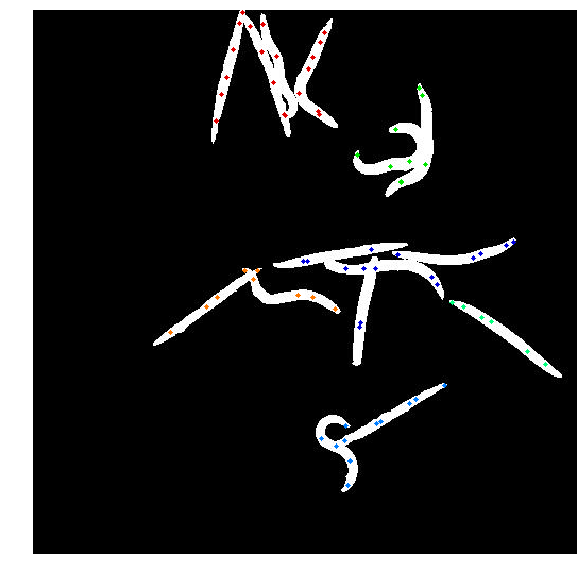
\includegraphics[width=9cm]{figure/chap4/rand_seed.png}
	  \bicaption
		{随机点采样的示例}
		{Example of random point sampling}
	  \label{fig:chap4:rand_seed}
	\end{figure}
\subsection{随机点的产生}
	随机点的产生直接影响线虫轮廓解析方法的效率,随机点的数量过大导致SingleOut-Net网络需要对大量的图像块处理,需要很大
	的计算量,从而导致解析一帧图像需要大量的时间。但随机点的数量太少,可能导致有些线虫的轮廓上没有随机点覆盖,
	这些线虫的轮廓将得不到解析。实验发现,直接在原图像中生成随机点的方式非常的低效,
	主要是因为前景像素只占原图中总像素的一小部分,大部分的随机点落在了背景里。
	本文提出一种高效的随机点产生方法。首先,提取原图中所有的轮廓,然后在每个轮廓的边缘上等距
	的采样一定数量的边界点,最后在边界点的邻域内再采样。这种随机点产生的方法只需要产生少量的随机点即可覆盖所有的
	线虫轮廓,最终采样的结果如图\ref{fig:chap4:rand_seed}所示。

\subsection{SingleOut-Net网络输出后处理}
	图\ref{fig:chap4:singleout}显示了利用训练好的SingleOut-Net网络对部分图像块处理的结果。从图中可以看出SingleOut-Net
	网络成功地将位于图片中央的线虫轮廓从周围的线虫轮廓中分离出来。经过二值化等后处理步骤后,再用轮廓提取算法即可得到所有图像块
	对应的中央线虫的轮廓。
	但由于在随机点生成的过程中同一个线虫轮廓上可能包含
	多个随机点,所以在SingleOut-Net输出的结果中,同一个线虫的轮廓可能出现了多次。通过计算两个线虫轮廓在原图坐标中面积的
	重合度可以判定这两个轮廓是否表示同一个线虫,当两个轮廓的面积重合度大于一个设定的阈值时,则只需保留其中的一个轮廓。当一个轮廓完全被另一个轮廓包含时,则保留
	轮廓面积较大的轮廓。过滤掉重复的轮廓以及不完整的轮廓后即可得到解析的结果,最终的解析结果示例
	如图\ref{fig:chap4:parser}所示。
	\begin{figure}[!h]
	  \centering
	  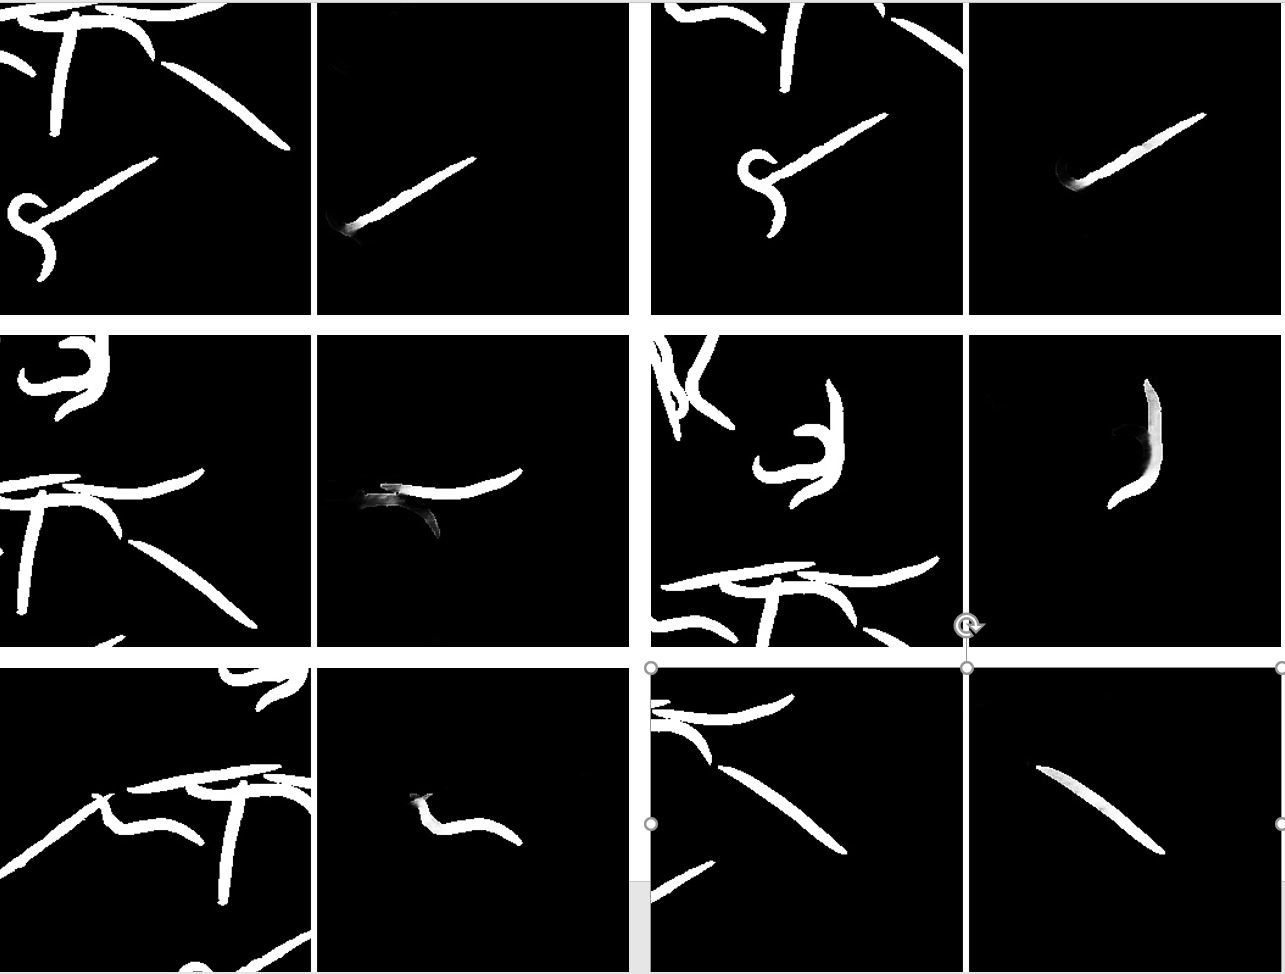
\includegraphics[width=10cm]{figure/chap3/singleout.jpg}
	  \bicaption
		{SingleOut-Net网络的输入输出示例}
		{Example of input and output of SingleOut-Net}
	  \label{fig:chap4:singleout}
	\end{figure}

	\begin{figure}[!htb]
	  \centering
	  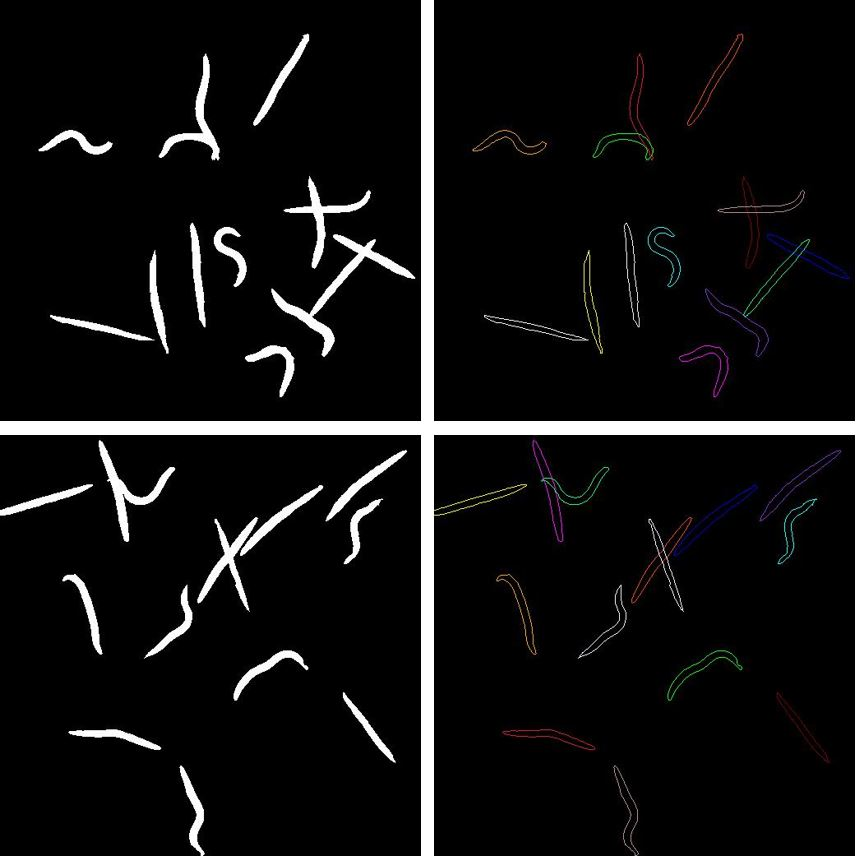
\includegraphics[width=10cm]{figure/chap4/Parser_Worms5.jpg}
	  \bicaption
		{多线虫轮廓解析结果}
		{Parser result of C.elegans contour}
	  \label{fig:chap4:parser}
	\end{figure}

\subsection{数据集的制作}
\label{dataset}
	SingleOut-Net网络的训练需要大量标定的数据集,本文采用了人工生成的数据集来训练网络的模型参数,
	数据集的制作流程如图\ref{fig:chap4:dataset}所示。
	BBBC010线虫数据集\cite{Ljosa2012Annotated}由马萨诸塞州综合医院Fred Ausubel教授的实验室采集并发布,
	该数据集中包含1407张经过前景背景分割的单线虫二值化图像。数据集制作的第一步需要从BBBC010数据集中
	提取所有单线虫的轮廓得到一个线虫的轮廓库(库中包含1407个不同姿势和大小的单线虫轮廓)。然后从单线虫的轮廓库中随机地选取一个线虫轮廓在一个
	分辨率为$256\times256$的背景图(像素值全为零)的中央画出。这一步得到的图作为网络训练的标签。继续从
	线虫轮廓库中随机选取若干个线虫的轮廓并在标签图像中随机的画出。至此,便得到了SingleOut-Net网络
	训练的的输入图像以及对应的
	标签。为了加快网络的收敛速度,本文将数据集的输入以及对应的标签图像归一化到$0\sim1$范围内,
	并加入一定量的高斯白噪声。
	通常数据集的多样性可以使神经网络学习到更多的模式,从而使网络具有更好的泛化能力。
	为了进一步增强数据集的多样性,本文对每个随机选取的单线虫轮廓进行随机的缩放和随机的旋转操作。
	\begin{figure}[htb]
	  \centering
	  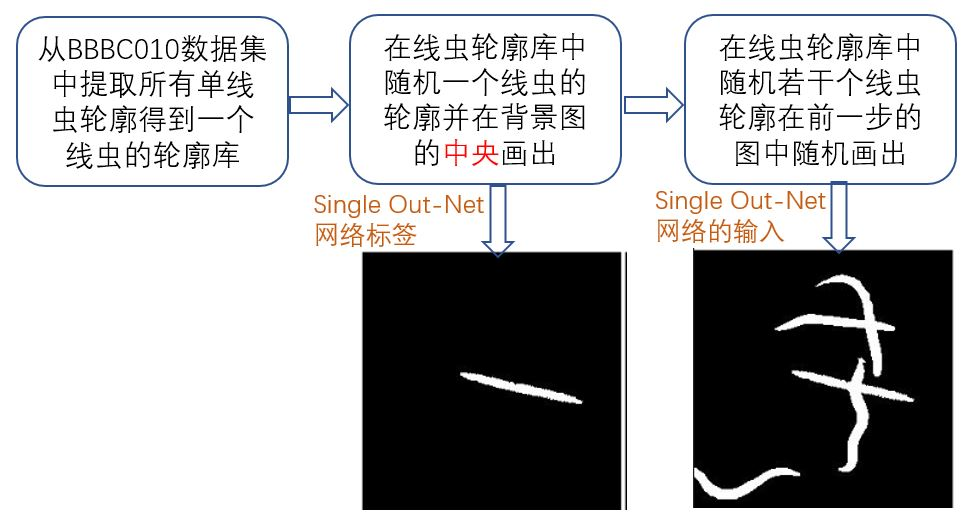
\includegraphics[width=12cm]{figure/chap4/dataset.jpg}
	  \bicaption
		{SingleOut-Net网络训练数据集的制作流程}
		{The production process of  training dataset for singleout-net network}
	  \label{fig:chap4:dataset}
	\end{figure}
\subsection{网络结构的设计}
\label{archtecture}
\begin{figure}[htb]
	  \centering
	  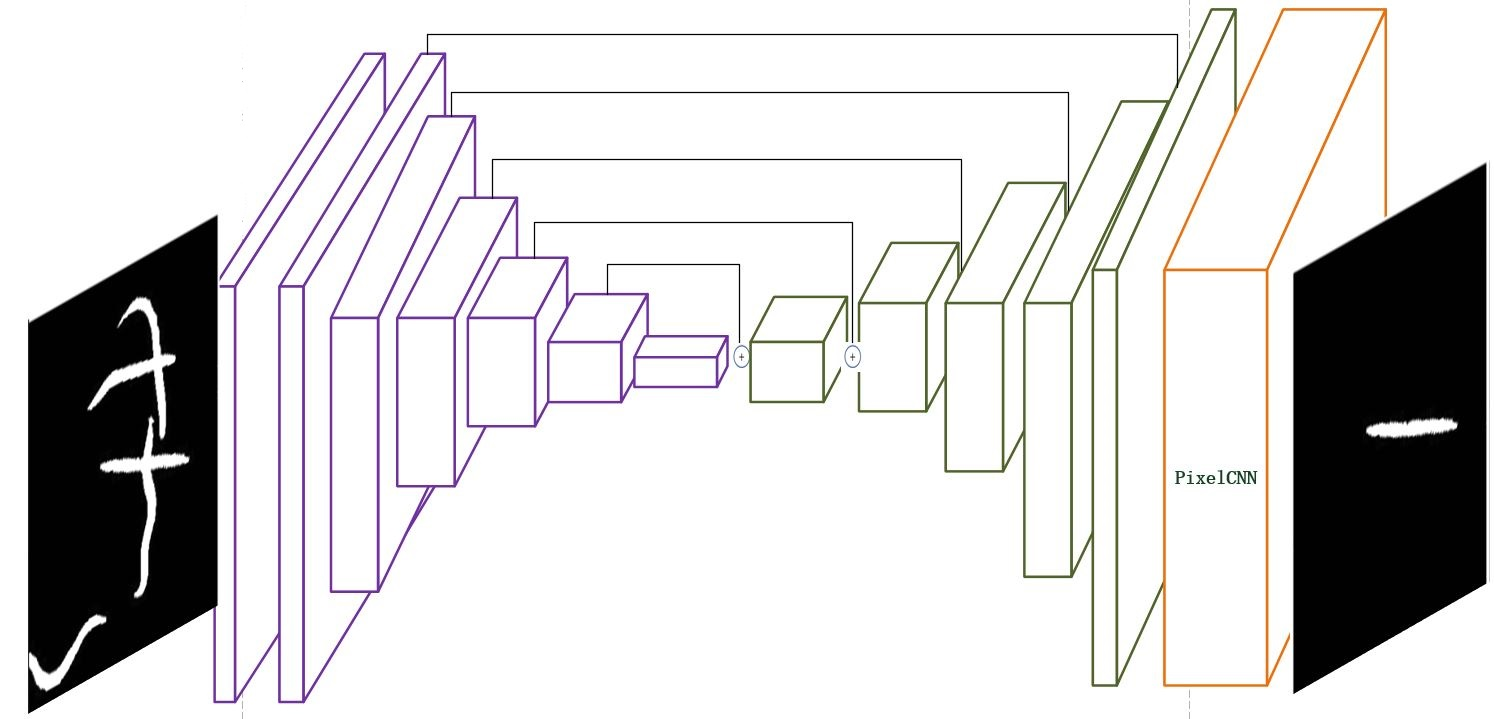
\includegraphics[width=14cm]{figure/chap4/arch1.jpg}
	  \bicaption
		{SingleOut-Net网络架构}
		{Architecture of SingleOut-Net}
	  \label{fig:chap4:netarch}
	\end{figure}
	如图\ref{fig:chap4:netarch}所示是SingleOut-Net的网络结构。网络的输入为$256\times256\times1$的张量,
	输出也为相同尺寸的张量,整个网络架构由两个模块级联构成。
	第一个模块为一个类似于U-Net网络\cite{ronneberger2015u}的卷积模块,在整个网络架构中
	相当于一个编码器。图中的方块都表示本章\ref{subsec:arch-design}节介绍的残差连接单元。第一个卷积模块包含两条路径,分别为降采样路径和
	上采样路径。降采样路径上每经过一个残差连接模块后面都连接一个降采样层,
	降采样层将输入张量的尺寸减小一倍同时将通道数扩大一倍。
	降采样层通过一个卷积层实现,其卷积核的大小为$2\times2$步长为2,卷积后紧跟着的是Batch Normalization 层
	和激活函数层。由于Relu函数\cite{xu2015empirical}具有克服梯度消失和加快网络收敛等优势,这里使用了Relu激活函数。
	上采样路径与降采样路径类似,只不过将降采样层换成上采样层。上采样层通过反卷积实现,其卷积核大小为$2\times2$步长为2。
	在图\ref{fig:chap4:netarch}中,上采样层的输入由两部分构成,
	分别为降采样路径中相同分辨率的张量和上采样路径中前面的张量,图中的加号表示张量的相加操作。
	第二个卷积模块为PixelCNN\cite{van2016conditional}模块,将其作为解码器。PixelCNN网络由Deepmind于2016年提出并用于
	条件图像生成,可以生成非常逼真的图像。本文将其应用在SingleOut-Net网络中作为解码器来生成中央线虫的图像。最后通过一个$1\times1$
	的卷积将特征通道数变为输出图像的通道数,并通过Sigmoid激活函数将输出的数值限制在$0\sim1$范围内。最终的输出是一个通道数为1
	的概率图,概率图中每一个像素值的大小表示该像素属于中央线虫轮廓的概率。

\subsection{评价指标}
	
\subsubsection{评价指标}
	为了更好的对不同的网络架构进行量化分析和性能比较,因此需要选取一些评价指标。本文提出的SingleOut-Net网络
	用于判别图像中每个像素是否属于中央线虫轮廓像素,所以是一个像素二分类网络。本文将像素分类误差作为网络评价指标,
	像素分类误差由公式\ref{eq:metrics}表示。
	\begin{equation}
		\text{像素误差} =1- \frac{\text{被正确分类的像素数目}}{\text{总的像素数目}} \label{eq:metrics}
	\end{equation}
\subsection{网络的训练}
	
	根据\ref{dataset}节介绍的数据集生成方法,可以生成任意大小的训练集。但为了节省内存开销,本文采用了训练集动态生成的方法
	,即在训练阶段每个minibatch的样本图片都是动态生成的。但动态生成训练样本需要一定的时间开销,从而使网络训练时间变长。为了缩短网络训练时间以及在限定
	时间内探索更优的网络架构,本文将数据生成和网络训练这两个任务并行,即用一个专门的线程负责数据集的生成。另外为了比较
	不同网络架构的性能,测试集的样本应该保持不变,而本文中的数据集是动态随机生成的。为了获得一个不变的测试集,在网络训练和模型测试阶段,本文分别采用了
	两个不同的随机数种子初始化随机数生成器。
		\begin{figure}[!b]
	  \centering
	  \includegraphics[width=13cm]{figure/chap4/loss1.jpg}
	  \bicaption
		{网络训练过程中训练损失随epoch数的变化}
		{The change of training loss with epoch number in the process of network training}
	  \label{fig:chap4:loss}
	\end{figure}
	
	神经网络模型的训练分为前向传播、反向传播和权值更新三个步骤。batchsize作为一个重要的超参数,其决定将多少样本作为一个整体估计梯度下降的方向。如果将其设置得过大,
	会导致网络模型很难跳出局部最小值点;如果设置得过小,则很难获得一个准确的梯度下降方向,
	在这里batchsize设置为4。
	神经网络的优化算法大致可以分为三大类:基于一阶微分的最优化方法(随机梯度下降)、基于二阶微分
	的最优化方法(牛顿法)以及基于二阶微分近似的方法(AdaDelta算法\cite{zeiler2012adadelta}和Adam算法\cite{kinga2015method}等)。随机梯度下降的最优化方法计算量
	最小,但网络的收敛速度慢。牛顿法由于利用了二阶梯度信息,与其他的最优化方法相比具有更好的收敛性能,但由于要计算
	Hessian矩阵所以计算量很大。于是研究者们提出了很多基于二阶微分的近似方法,这些最优化方法是计算量和
	收敛性能的一个折中。本文采用了Adam最优化方法优化网络模型并将学习率设置为0.0002,将交叉熵损失作为训练的损失函数。
	训练40个epoch(每个epoch包含1000个batch)后网络已经完全收敛,
	图\ref{fig:chap4:loss}表示损失函数随epoch数的增加而下降,经过 20个epoch后
	网络已经基本收敛。

	
	为了观察网络训练过程中SingleOut-Net网络性能的变化,本文对网络模型每隔100次迭代进行一次测试,图\ref{fig:chap4:progress}
	显示了网络训练过程中网络模型测试的结果。从图中可以看出随着网络模型迭代次数的增加,SingleOut-Net网络逐渐学会过滤掉非中央
	线虫的轮廓,只保留中央线虫的轮廓。
		\begin{figure}[htb]
	  \centering
	  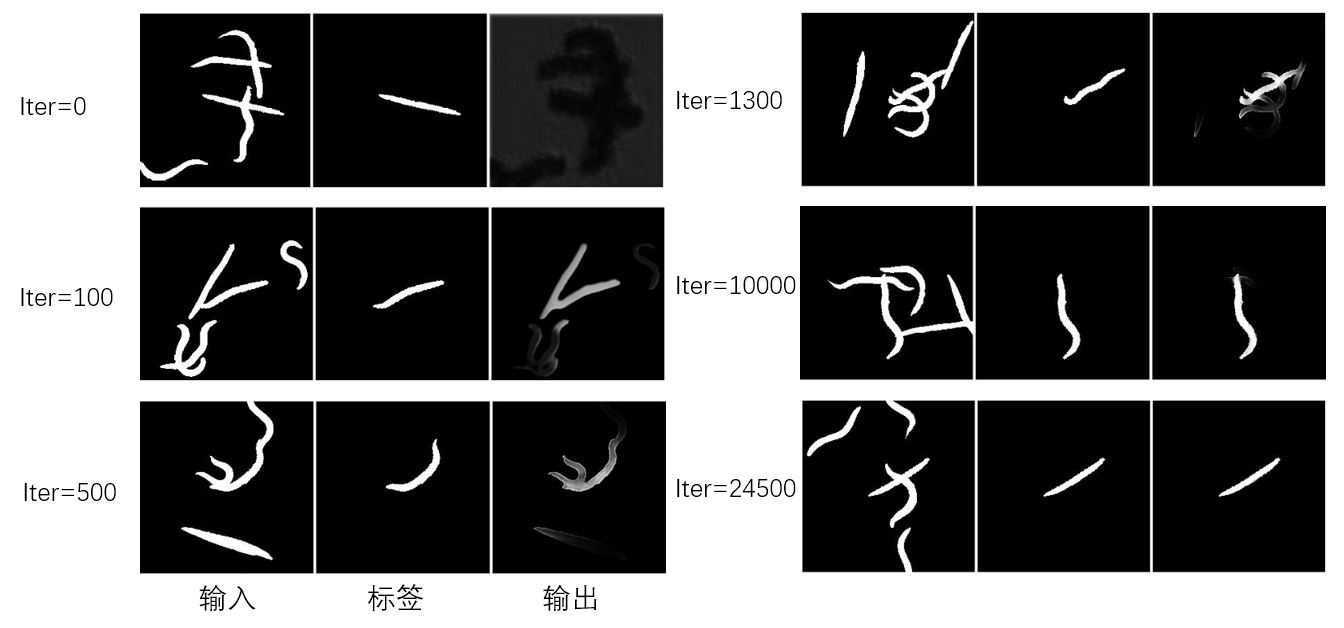
\includegraphics[width=15cm]{figure/chap4/progress.jpg}
	  \bicaption
		{网络训练过程中模型测试结果}
		{Model test results during network training}
	  \label{fig:chap4:progress}
	\end{figure}
\subsection{测试结果与分析}
	 在\ref{archtecture}节,本文介绍了SingleOut-Net的网络架构,由两个卷积模块构成编解码器结构。为了
	 便于区分,本文将其命名为模型一。为了分析这种编解码结构的网络性能,
	 本文分别从像素误差、模型复杂度和推断时间三个方面考察了
	 pixelCNN卷积模块对整个网络架构的影响。由于pixelCNN网络模块的输入和输出的尺寸保持不变,
	 所以将pixelCNN模块移去后,用一个$1\times1$的卷积将编码器模块输出的通道数变成网络最终输出的通道数。
	 将这种没有pixelCNN模块的网络架构命名为模型二。两个模型的性能比较如表\ref{tab:performance}所示。
	 从表中可以看出pixelCNN网络模块可以显著地降低像素误差(10倍下降),但同时由于增加了网络的深度,使得网络在推断单张图片所消耗
	 的时间变长。
\begin{table}[!hpb]
	\centering
	\bicaption
    {两种网络模型性能的比较}
    {Comparison of performance of two network models}
	\label{tab:performance}
	\begin{tabular}{p{75pt}p{75pt}p{75pt}p{75pt}}
	\toprule
	网络模型 & 像素误差 & 模型大小 & 推断时间 \\
	\midrule
	模型一 &  0.00521\% & 46.8Mb & 31ms \\
	模型二 & 0.00045\% & 48.9Mb & 100ms \\
	\bottomrule
\end{tabular}
\end{table}
\section{线虫轮廓的跟踪}
	由于秀丽隐杆线虫通体透明,跟踪起来比较困难,本文采用了一种简单有效的跟踪策略。首先经过
	线虫前景轮廓分割和线虫轮廓解析等步骤后,可以得到每一帧图像里所有线虫的轮廓。由
	公式\ref{eq:m}和公式\ref{eq:xy}可以计算出轮廓的重心坐标。
	\begin{equation}
		m_{ji}=\sum_{x,y}I_{x,y}x^iy^j \label{eq:m}
	\end{equation}
	\begin{equation}
		\vec{x}=\frac{m_{10}}{m_{00}},\quad \vec{y}=\frac{m_{01}}{m_{00}}\label{eq:xy}
	\end{equation}
	假设当前帧有n个线虫轮廓,上一帧
	图像有m个线虫轮廓,由每个轮廓的重心坐标可以计算出相邻两帧图像线虫轮廓重心之间的距离,
	从而得到一个$n\times m$的距离矩阵用公式\ref{eq:matrix}
	表示。
		\begin{equation}
                        D=\left[
                \begin{matrix}
                 d_{11}      & d_{12}      & \cdots & d_{1m}      \\
                 d_{21}      & d_{22}      & \cdots & d_{2m}      \\
                 \vdots & \vdots & \ddots & \vdots \\
                 d_{n1}      & d_{n2}      & \cdots & d_{nm}      \\
                \end{matrix}
                \right]\label{eq:matrix}
    \end{equation}
	% \begin{figure}[t]
	  % \centering
	  % 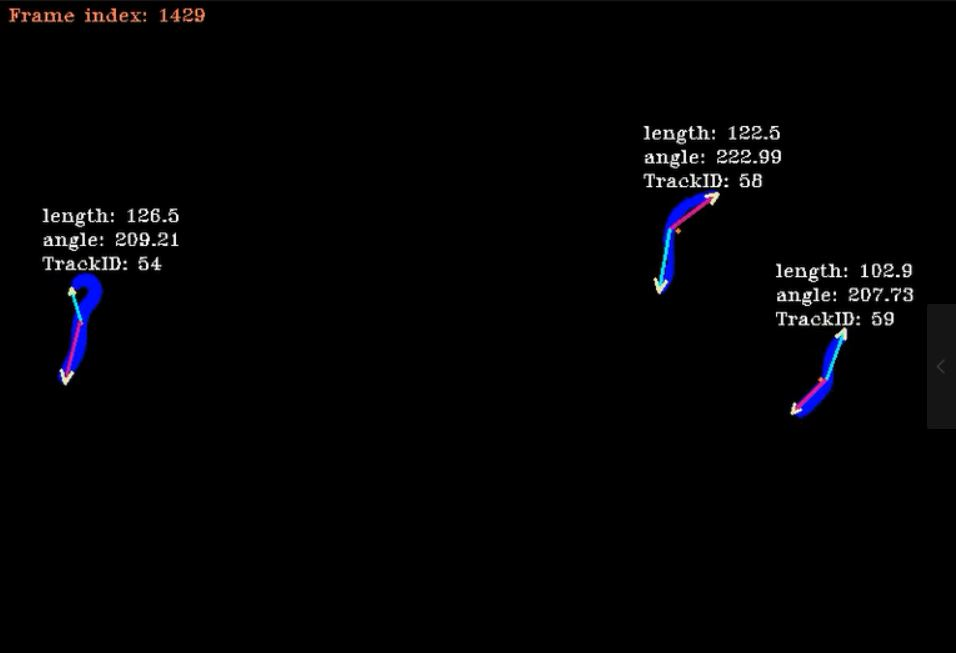
\includegraphics[width=9cm]{figure/chap5/tracking.jpg}
	  % \bicaption
		% {线虫跟踪的结果}
		% {The result of worm tracking }
	  % \label{fig:track}
	% \end{figure}
	矩阵中$d_{ij}$表示当前帧图像中的第i个轮廓的重心到上一帧图像中第j个轮廓的重心之间的距离。通过
	公式\ref{eq:min}可以得到相邻两帧图像中线虫轮廓之间的对应关系。即如果相邻两帧图像中两个
	轮廓重心之间的距离最短,则可以认为是同一个线虫的轮廓。在线虫跟踪过程中,每个线虫用一个TrackID来标识,
	不同的TrackID代表不同的线虫。
		\begin{equation}
        index(i)=\mathop{\arg\min}_{j} d_{ij}\label{eq:min}
		\end{equation}
	但事实上由于线虫轮廓分割的不完整以及图像噪声的影响
	,这一策略往往会失效。因此,为了提高线虫轮廓跟踪的鲁棒性,在轮廓匹配的过程中本文增加了两个约束条件:
	\begin{itemize}
	  \item 相邻两帧图像中同一只线虫的轮廓面积相对变化应该小于一个阈值。
	  \item 根据线虫运动的最大速度限制,同一只线虫在相邻两帧图像中轮廓重心的移动距离应该小于一个阈值。
	\end{itemize}
	当这两个条件之一不满足时,则认为跟踪丢失,此时应该分配一个新的trackID给当前的轮廓。
	算法\ref{algo:initial_track}和算法\ref{algo:worm_track}描述了线虫跟踪算法的实现思路。
\begin{algorithm}
\caption{线虫轮廓跟踪初始化算法}
\label{algo:initial_track}
\begin{algorithmic}[1]
	\Require $Worm\_data$双重列表,$Worm\_data[i][j]$表示第$i$帧图像中第$j$只线虫。
	\Ensure 输出$trackID$
	\Function {Initiate\_tracking}{$Worm\_data$}
		\State $FirstFrame\_WormData \gets Worm\_data[0]$
		\For{$i = 0 \to FirstFrame\_WormData.length-1$}
			\State $cur\_worm \gets FirstFrame\_WormData[i]$
			\State $cur\_worm.trackID \gets GetNewTrackID()$
		\EndFor
\EndFunction
\end{algorithmic}
\end{algorithm}

\begin{algorithm}[H]
\caption{线虫轮廓跟踪算法}
\label{algo:worm_track}
\begin{algorithmic}[1]
	\Require $Worm\_data$双重列表,$Worm\_data[i][j]$表示第$i$帧图像中第$j$只线虫。$\delta$和$\sigma$均表示约束条件中的阈值。
	\Ensure 输出$trackID$
	\Function {Worm\_tracking}{$Worm\_data$}
		\State $Initiate\_tracking(Worm\_data)$
		\For{$frame\_index = 1 \to Worm\_Data.length-1$}
			\State $PreFrame\_WormData \gets Worm\_Data[frame\_index-1] $
			\For{$worm\_index =0 \to Worm\_Data[frame_index].length-1$}
				\State $cur\_worm \gets Worm\_Data[frame\_index][worm\_index]$
				\State $dist\_array \gets Compute\_distance(cur\_worm,PreFrame\_WormData)$
				\State $min\_index \gets Get\_min\_index(dist\_array)$
				\State $Nearest\_worm \gets PreFrame\_WormData[min\_index]$
\algstore{WormTracking}
\end{algorithmic}
\end{algorithm}
\begin{algorithm}[H]
\begin{algorithmic}[1]
\algrestore{WormTracking}
				\If{$\small{\frac{|Nearest\_worm.Area-cur\_worm.Area|}{Nearest\_worm.Area}<\delta \quad \text{and}  \quad dist\_array[min\_index]< \sigma}$}
					\State $cur\_worm.trackID \gets Nearest\_worm.trackID$
				\Else
					\State $cur\_worm.trackID \gets GetNewTrackID( )$
				\EndIf
			\EndFor
		\EndFor
\EndFunction
\end{algorithmic}
\end{algorithm}
\section{线虫的特征提取}
	线虫从头部到尾部两边近似等距的分布着23-24块肌肉,其头部和尾部各占其总长度的$1/6$,因此线虫
	身体的自由度为24。当用轮廓来描述线虫的形态时,在其轮廓四周采样49个点足以描述线虫所有形态。
	当对线虫进行特征计算时(如:计算线虫摆动频率和运动速度等),通常是利用线虫轮廓中间的脊线进行计算。
	因此需要提取线虫轮廓的中线然后采样24个点用于特征计算。下面将首先对线虫轮廓中间脊线提取算法进行介绍,
	然后介绍线虫摆动频率的计算。
\subsection{线虫轮廓中间脊线提取}
	在得到线虫的轮廓后,将轮廓上的坐标按顺时针排列即可得到一个坐标点的循环列表。
	将轮廓周长的$1/48$作为一个单位边,
	对于线虫轮廓边缘的任意一点而言,在其两边都可以找到一个距离为单位边长度的相邻点,这三点所成角的补角与该点的曲率成正比,因此
	可以用于近似曲率的计算。由于其头部和尾部的曲率往往比身体的其他部分要尖锐,所以如果将像素索引作为横坐标,
	曲率作为纵坐标,则这条曲线上将会出现两个波峰如图\ref{fig:qulv}所示,分别对应线虫的头部和尾部。
	由此便可定位到线虫的头部和尾部,另外线虫的头部
	曲率一般小于尾部的曲率,两个波峰中比较低的波峰对应的横坐标为线虫头部的坐标,
	另一个波峰对应线虫尾部的坐标。
	线虫头部和尾部将线虫轮廓分为两边。在其中一条边上找到所有距离另一条边最近的对应点。
	两条边上两对应点的中点构成线虫的中间脊线,线虫轮廓中间脊线的长度定义为线虫的体长。
	\begin{figure}[h]
	  \centering
	  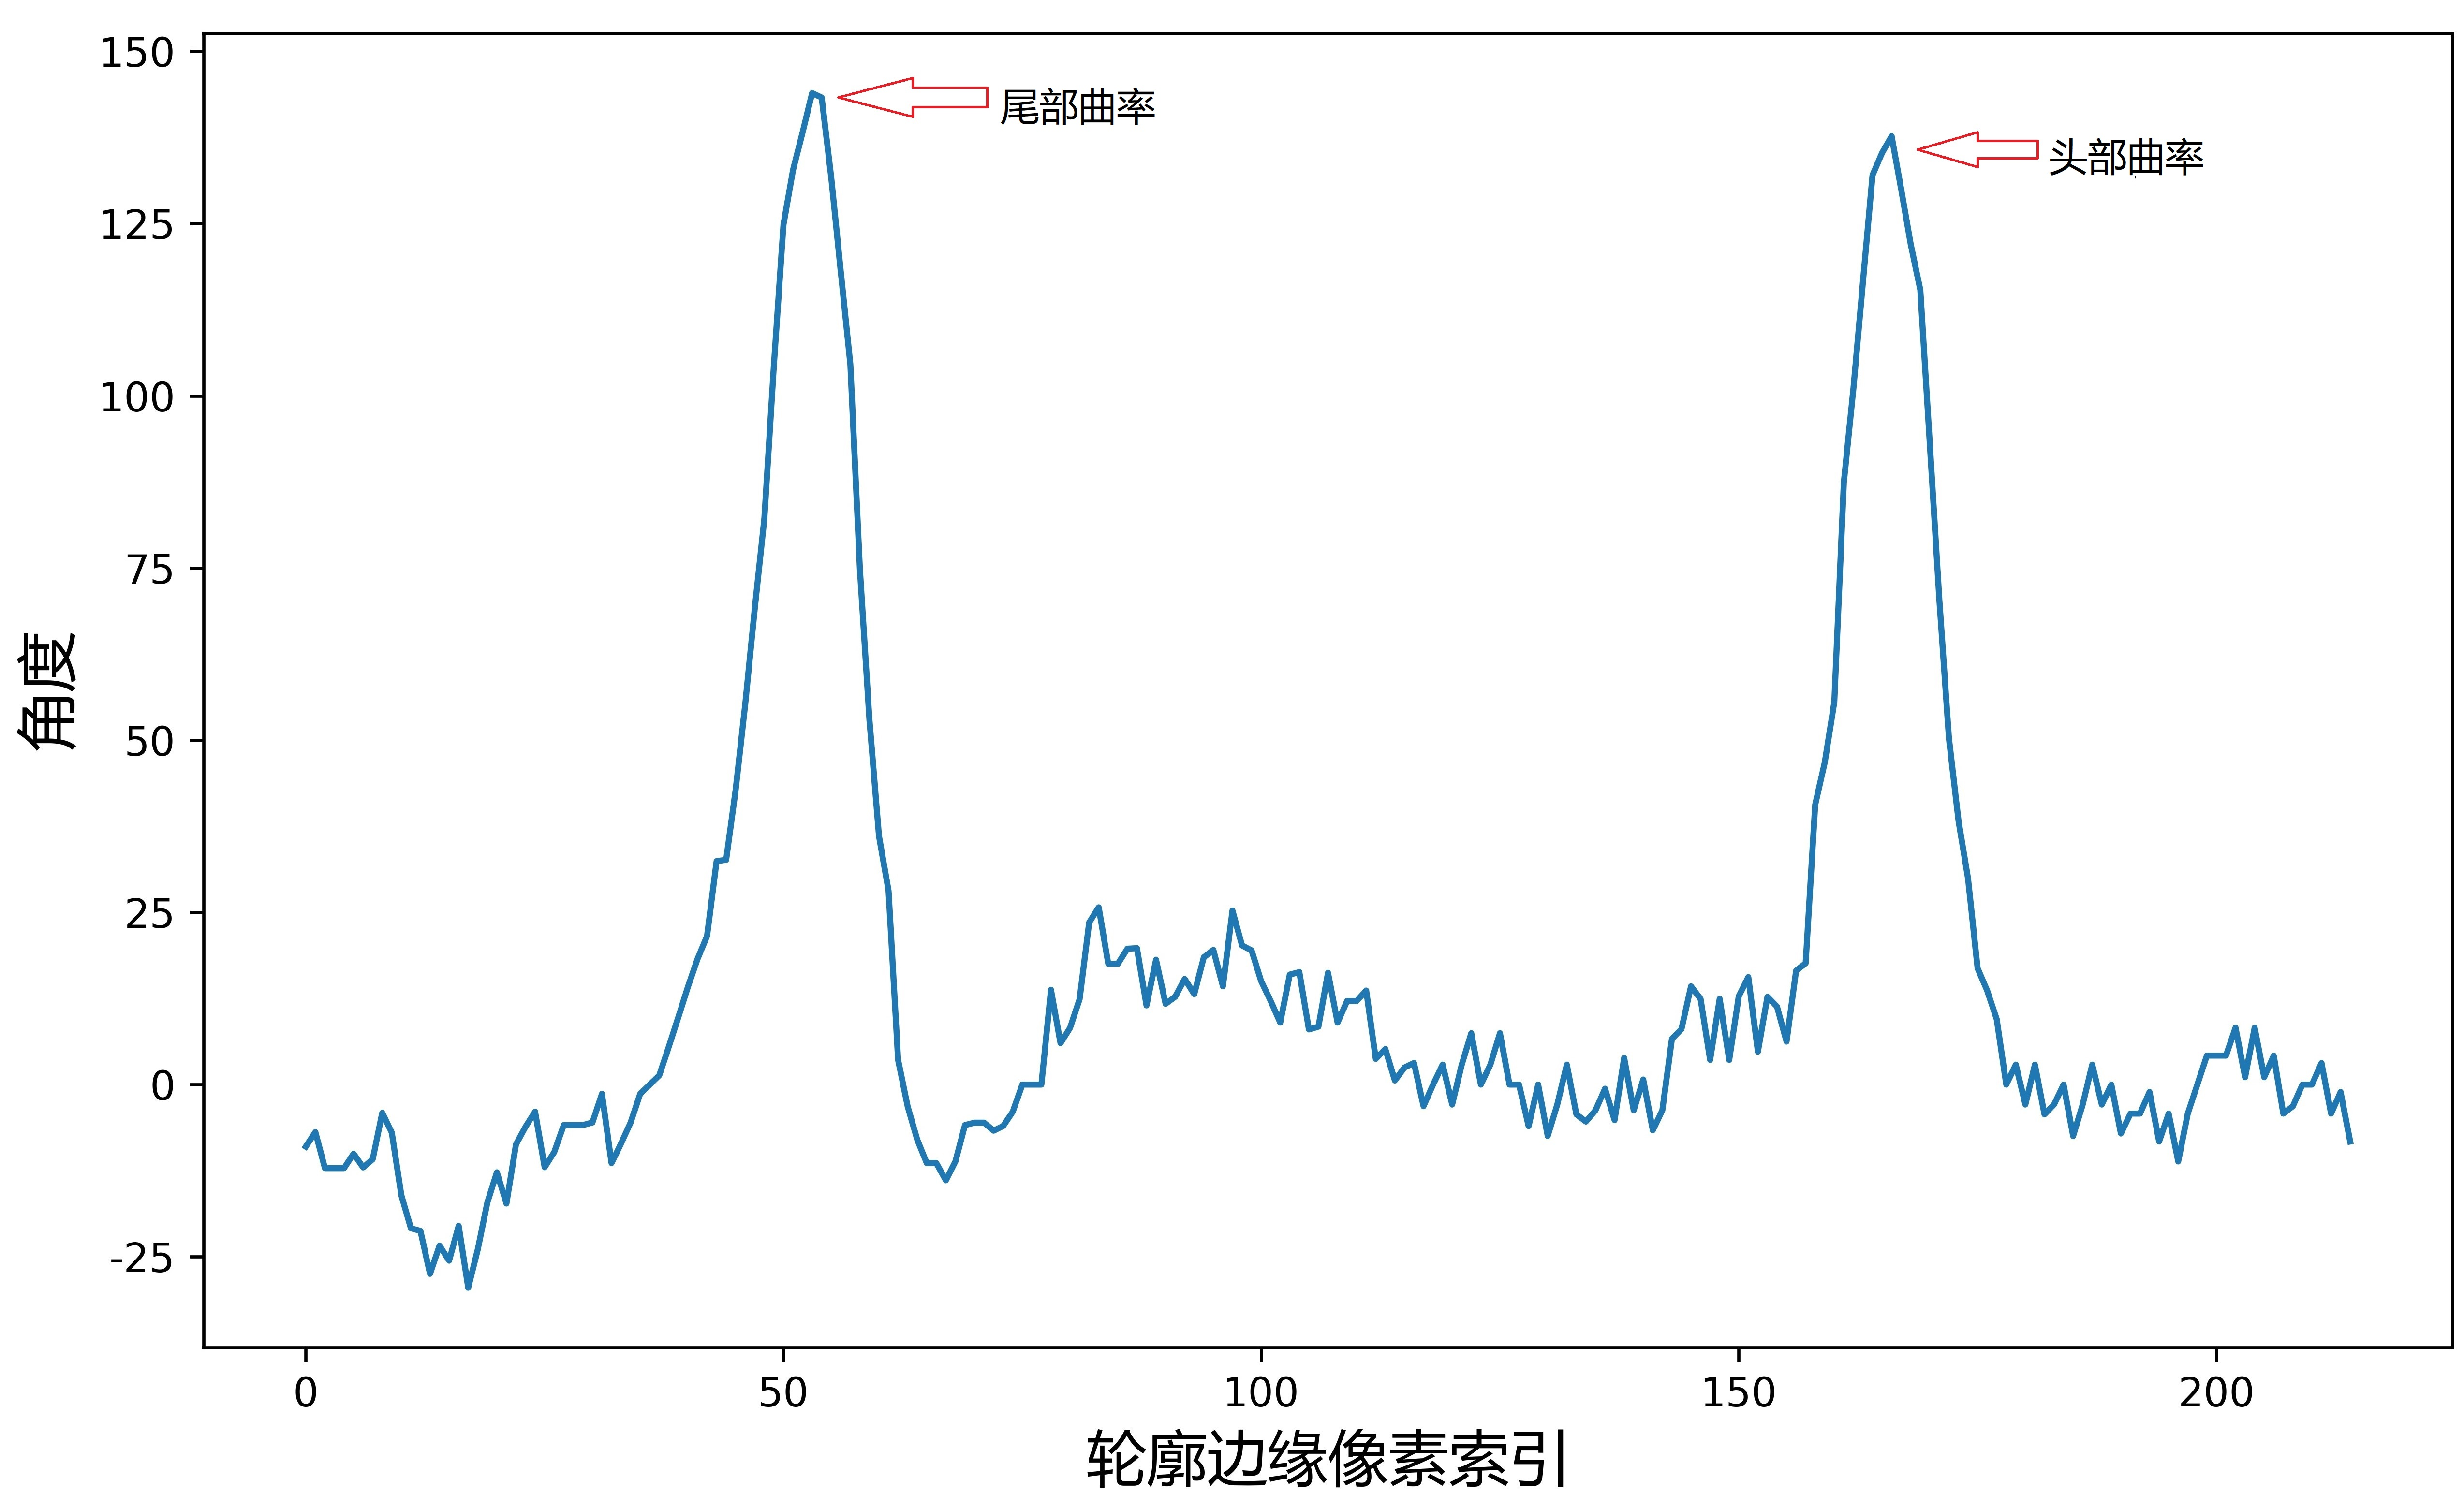
\includegraphics[width=14cm]{figure/chap5/cuvature.jpg}
	  \bicaption
		{轮廓曲率的变化}
		{Change in contour curvature}
	  \label{fig:qulv}
	\end{figure}
\subsection{身体弯曲角度的计算以及摆动频率的估计}
	在很多毒理实验中,线虫的摆动频率经常作为一个重要的生理指标用于表征线虫的活跃程度\cite{Wang2008Assessment}。
	为了计算线虫的摆动频率, 我们定义一个衡量身体弯曲程度的夹角,由线虫头部、尾部和轮廓脊线的中点三点所成角定义为
	身体弯曲角。线虫在爬行和游动的过程中,身体弯曲角会在$180^\circ$C左右振荡,
	振荡的频率定义为线虫摆动的频率。在时刻$t_0$,对区间$(t_0-\Delta t,t_0+\Delta t)$中弯曲角信号做FFT变换,假设其幅度最大值对应的横坐标
	为n,则线虫在$t$时刻的瞬时摆动频率由公式\ref{eq:freq}得出。
	\begin{equation}
        \text{Swing frequency}=\frac{frame\_rate*n}{2*\Delta t} \label{eq:freq}
	\end{equation}
		
% \begin{figure}[!htp]    
% % \begin{minipage}[t]{0.5\linewidth}%设定图片下字的宽度,在此基础尽量满足图片的长宽    
	% \centering    
	% 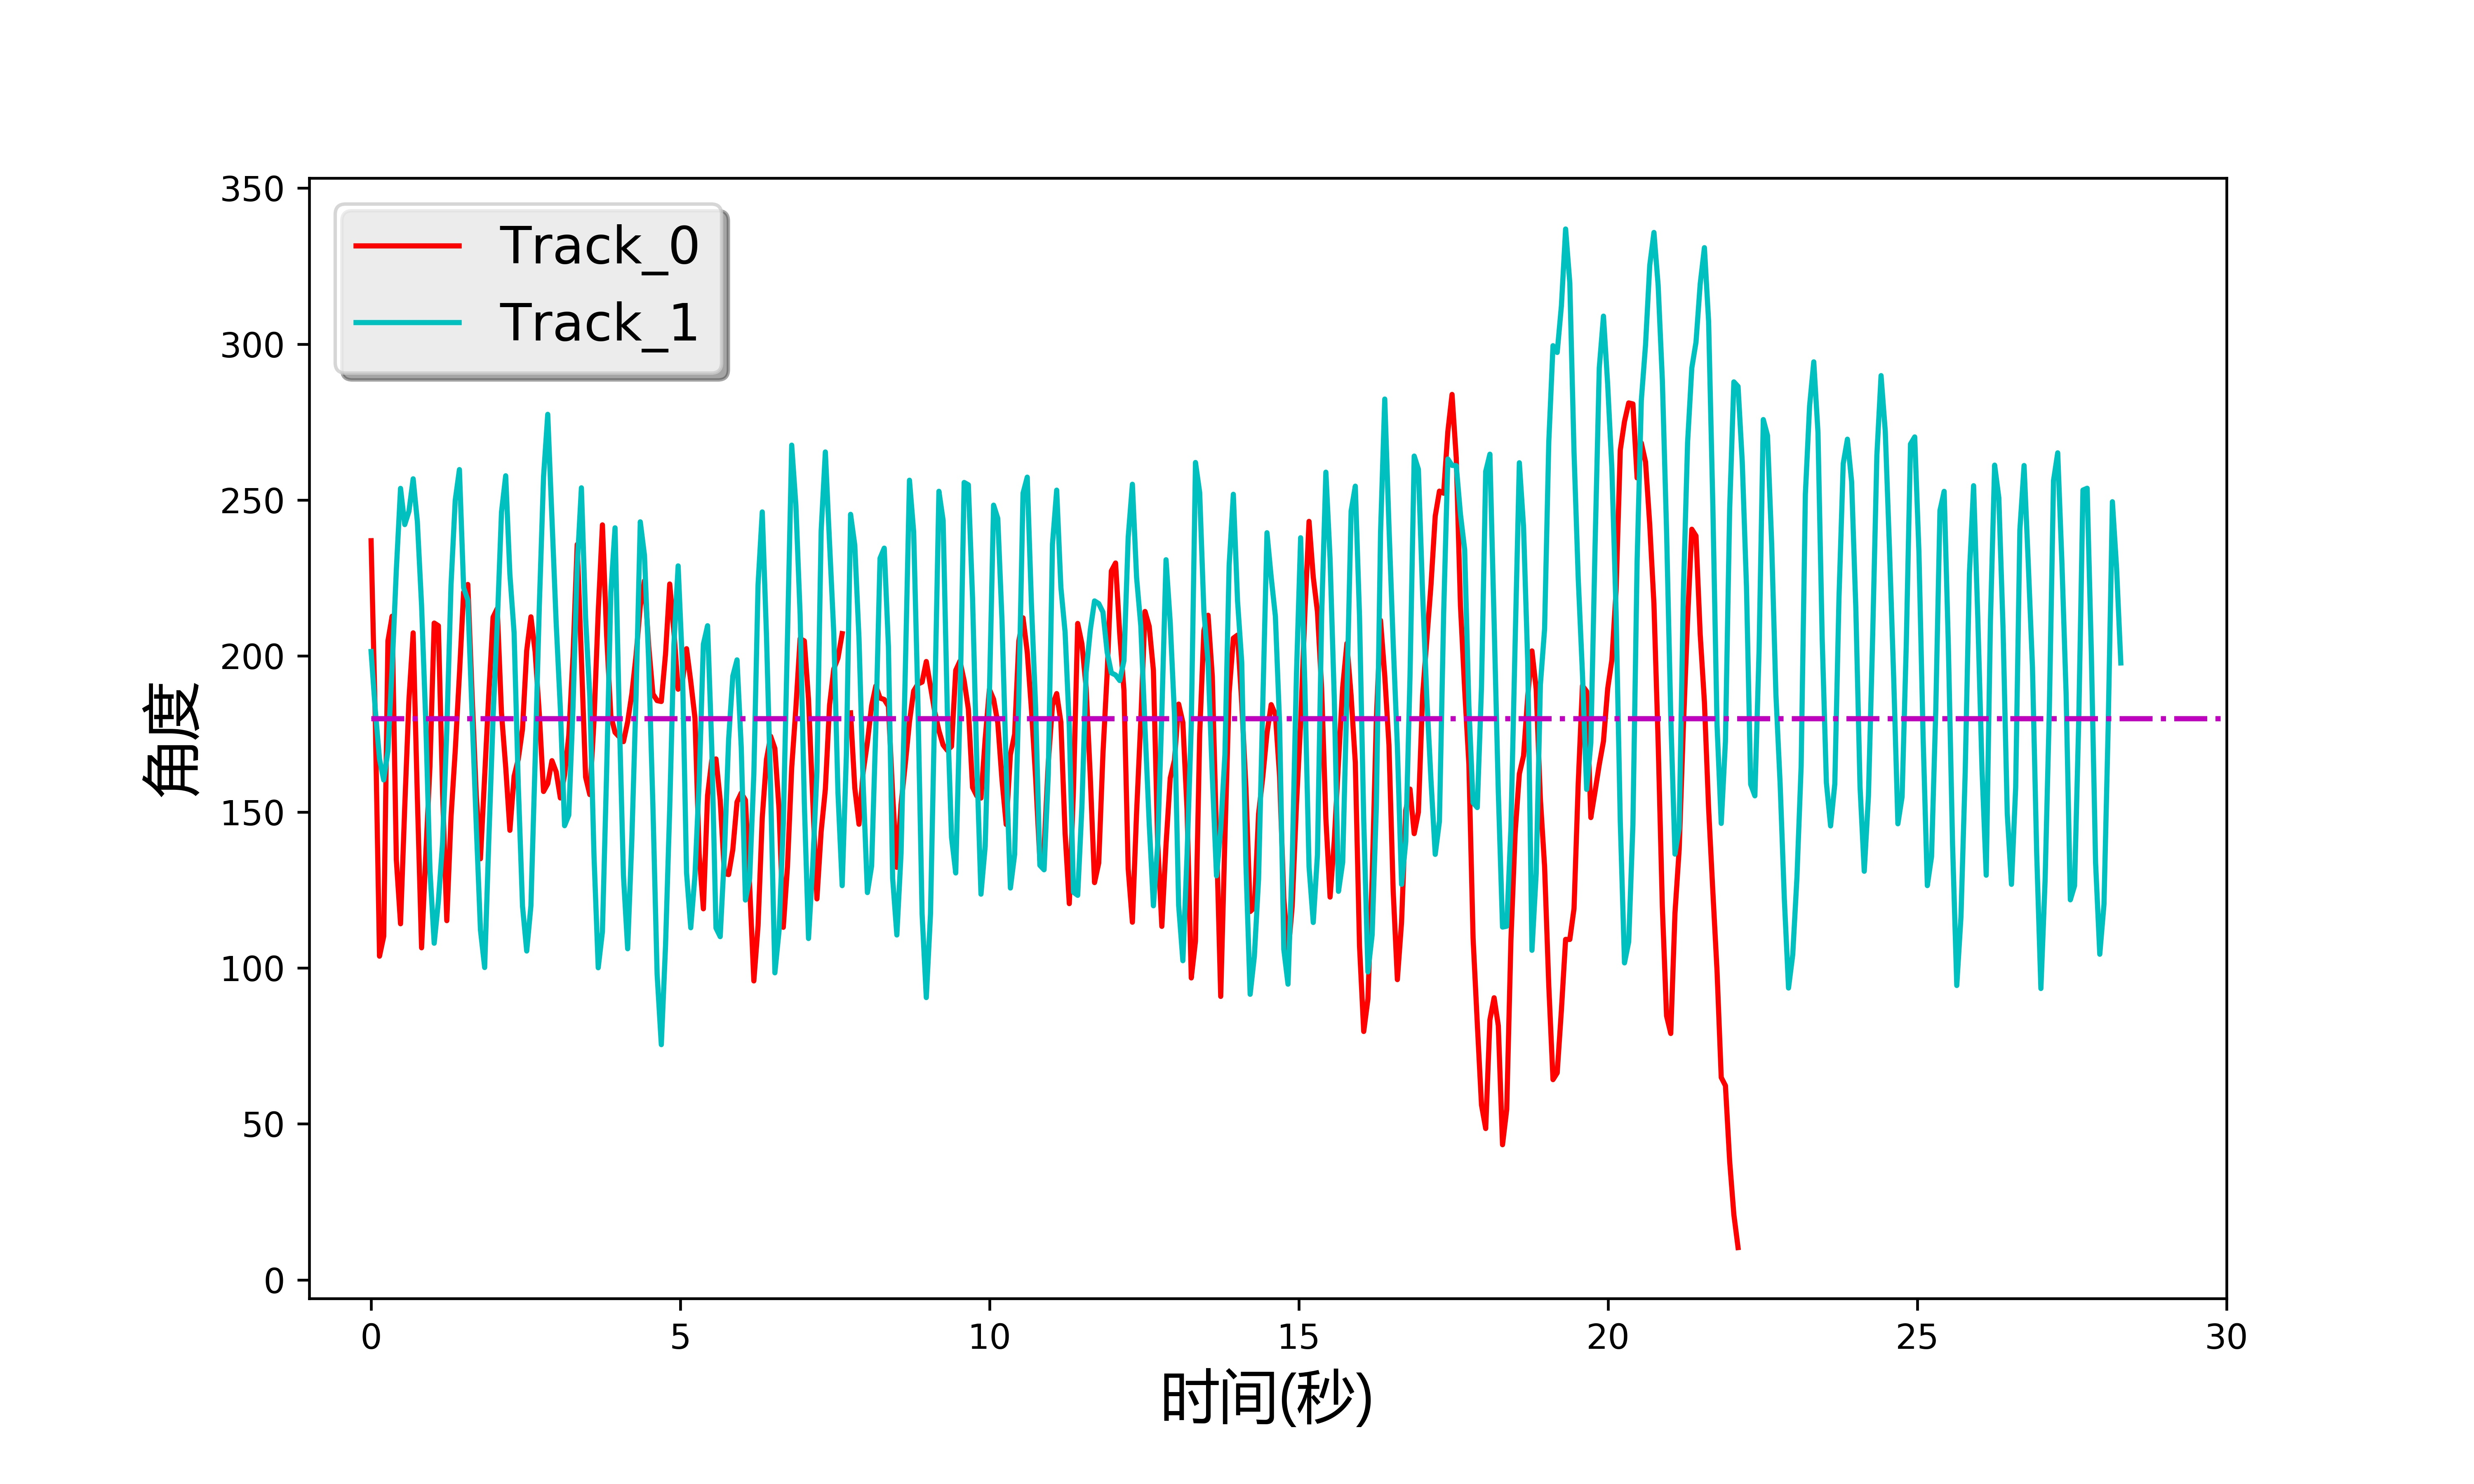
\includegraphics[width=1\linewidth]{figure/chap3/angle.jpg}    
% \bicaption{线虫弯曲角度的变化}
% {Change in the bending angle of C.elegans}%n张图片共享的说明
% \label{fig:angle}
% \end{figure}
\section{本章小结}
	本章为药物筛选平台的软件部分,针对线虫药物筛选实验中的自动化视频分析和特征提取的需求。本文
	提出了“前景轮廓分割——轮廓解析——轮廓跟踪——特征提取”的技术路线。并按照技术路线流程依次对各个
	部分进行了详细的介绍,本章的主要工作如下:
	\begin{enumerate}[label={(\arabic*)},font={\color{black!50!black}\bfseries}]
	  \item 针对传统的图像分割方法在线虫前景轮廓分割任务中存在的不足(如:鲁棒性不足、分割效果
	  不理想、线虫轮廓不连续等问题),本章提出了一种基于条件随机场模型的深度卷积分割算法。通过
	  实验对比分析,发现本章提出的分割算法能够显著改善线虫前景轮廓分割的效果,能够得到更加
	  连续的线虫轮廓,且与传统图像分割方法相比,该方法具有鲁棒性的优势。
	  \item 针对多线虫轮廓跟踪过程中多线虫轮廓相互纠缠导致无法辨识到单个线虫轮廓的问题,本章设计了
	  一个基于深度卷积的SingleOut-Net网络,通过生成的数据对其进行训练。并将两种网络架构
	  在网络性能、模型复杂度以及实时性三个方面进行了比较,实验结果显示本章提出的
	  轮廓解析方法能够有效地解析到单线虫的轮廓。
	  \item 基于线虫前景轮廓分割和轮廓解析的结果,本章提出了一种简单的基于最近邻匹配的
	  线虫轮廓跟踪算法,在线虫轮廓分割较为完整的情况下,能够实现线虫轮廓的鲁棒跟踪。
	  \item 基于线虫轮廓跟踪的结果,介绍了线虫中间脊线的提取和线虫摆动频率的计算方法。
	\end{enumerate}